%%%%%%%%%%%%%%%%%%%%%%%%%
% Dokumentinformationen %
%%%%%%%%%%%%%%%%%%%%%%%%%
\newcommand{\titleinfo}{Computational Algebra \& Numerical Analysis}
\newcommand{\authorinfo}{R. Koller, L. Schmid, S. Eicher, G. Danuser} % Do not remove any names! Initial authors stay first.
\newcommand{\versioninfo}{$Revision: 239 $ - powered by \LaTeX}

%%%%%%%%%%%%%%%%%%%%%%%%%%%%%%%%%%%%%%%%%%%%%
% Standard projektübergreifender Header für
% - Makros 
% - Farben
% - Mathematische Operatoren 
%
% DORT NUR ERGÄNZEN, NICHTS LÖSCHEN
%%%%%%%%%%%%%%%%%%%%%%%%%%%%%%%%%%%%%%%%%%%%%  
% Genereller Header
\documentclass[10pt,twoside,a4paper,fleqn]{article}
\usepackage[left=1cm,right=1cm,top=1cm,bottom=1cm,includeheadfoot]{geometry}
\usepackage[ngerman]{babel,varioref}
\usepackage[utf8]{inputenc}

% Pakete
\usepackage{amssymb}
\usepackage{amsmath}
\usepackage{bm} % Bold Math
\usepackage{fancybox}
\usepackage{graphicx}
\usepackage[usenames,dvipsnames,svgnames,table]{xcolor}
\usepackage{lastpage}
\usepackage{wrapfig}
\usepackage{fancyhdr}
\usepackage{hyperref}
\usepackage{verbatim}
\usepackage{pdflscape} % landscape
\usepackage{multirow} % zellen in tabellen verbinden
\usepackage{multicol}
\usepackage{slashbox} % getrennte zelle in tabelle
% \usepackage{array} % anordnung in tabellen
\usepackage{booktabs}

%%%%%%%%%%%%%%%%%%%%
% Generelle Makros %
%%%%%%%%%%%%%%%%%%%%
\newcommand{\formelbuch}[1]{$_{\textcolor{red}{\mbox{\small{S#1}}}}$}
\newcommand{\verweis}[2]{ {\small (siehe auch \ref{#1}, #2 (S. \pageref{#1}))
}}
\newcommand{\subsubadd}[1]{\textcolor{black}{\mbox{#1}}}
\newenvironment{liste}[0]{
	\begin{list}{$\bullet$}{\setlength{\itemsep}{0cm}\setlength{\parsep}{0cm} \setlength{\topsep}{0cm}}}
    {\end{list}}
    
\newcommand{\logd}[0]{\log_{10}}
\newcommand{\subsubsubsection}[1]{\textbf{#1}}

\newenvironment{aufzaehlung}[0]{
	\begin{enumerate}{\setlength{\itemsep}{0cm}\setlength{\parsep}{0cm}
	\setlength{\topsep}{0cm}}} {\end{enumerate}}    

\newcommand{\abbHeight}[3]{
	\begin{center}
		\includegraphics[height=#2]{./bilder/#1} \\
		#3
    \end{center}
}
%Kreis um Buchstabe,Zahl
\newcommand*\kreisS[2]{\unitlength1ex\begin{picture}(2.5,2.5)%
\put(0.75,0.75){\circle{3}}\put(0.7,0.7){\makebox(0,0){#1}}\end{picture}$^{\displaystyle \text{#2}}$}

\newcommand*\kreisM[2]{\unitlength1ex\begin{picture}(3.5,3.5)%
\put(0.75,0.75){\circle{4}}\put(0.7,0.7){\makebox(0,0){#1}}\end{picture}$^{\displaystyle ^{\displaystyle \text{#2}}}$}

\newcommand*\kreisB[2]{\unitlength1ex\begin{picture}(3.5,3.5)%
\put(0.75,0.75){\circle{5}}\put(0.7,0.7){\makebox(0,0){#1}}\end{picture}$^{\displaystyle ^{\displaystyle \text{#2}}}$}

\newcommand{\todo}[1]{\colorbox{red}{#1}}
\newcommand{\hilight}[1]{\colorbox{yellow}{#1}}

%\newcommand{\skriptsection}[2]{\section{#1 {\tiny Skript S. #2}}}
%\newcommand{\skriptsubsection}[2]{\subsection{#1 {\tiny Skript S. #2}}}
%\newcommand{\skriptsubsubsection}[2]{\subsubsection{#1 {\tiny Skript S. #2}}}
%\renewcommand{\skriptsection}[2]{\section{#1 {\tiny Schaum S. #2}}}
%\renewcommand{\skriptsubsection}[2]{\subsection{#1 {\tiny Schaum S. #2}}}
%\renewcommand{\skriptsubsubsection}[2]{\subsubsection{#1 {\tiny Schaum S. #2}}}
\newcommand{\skriptsection}[2]{\section{#1 \formelbuch{#2}}}
\newcommand{\skriptsubsection}[2]{\subsection{#1 \formelbuch{#2}}}
\newcommand{\skriptsubsubsection}[2]{\subsubsection{#1 \formelbuch{#2}}}

%%%%%%%%%%
% Farben %
%%%%%%%%%%
\definecolor{black}{rgb}{0,0,0}
\definecolor{red}{rgb}{1,0,0}
\definecolor{white}{rgb}{1,1,1}
\definecolor{grey}{rgb}{0.8,0.8,0.8}

%%%%%%%%%%%%%%%%%%%%%%%%%%%%
% Mathematische Operatoren %
%%%%%%%%%%%%%%%%%%%%%%%%%%%%
\DeclareMathOperator{\sinc}{sinc}
\DeclareMathOperator{\sgn}{sgn}



% Fouriertransformationen
\unitlength1cm
\newcommand{\FT}
{
\begin{picture}(1,0.5)
\put(0.2,0.1){\circle{0.14}}\put(0.27,0.1){\line(1,0){0.5}}\put(0.77,0.1){\circle*{0.14}}
\end{picture}
}


\newcommand{\IFT}
{
\begin{picture}(1,0.5)
\put(0.2,0.1){\circle*{0.14}}\put(0.27,0.1){\line(1,0){0.45}}\put(0.77,0.1){\circle{0.14}}
\end{picture}
}



%%%%%%%%%%%%%%%%%%%%%%%%%%%%
% Allgemeine Einstellungen %
%%%%%%%%%%%%%%%%%%%%%%%%%%%%
%pdf info
\hypersetup{pdfauthor={\authorinfo},pdftitle={\titleinfo},colorlinks=false}
\author{\authorinfo}
\title{\titleinfo}

%Kopf- und Fusszeile
\pagestyle{fancy}
\fancyhf{}
%Linien oben und unten
\renewcommand{\headrulewidth}{0.5pt} 
\renewcommand{\footrulewidth}{0.5pt}


\fancyhead[L]{\titleinfo{ }- Summary}
%Kopfzeile rechts bzw. aussen
\fancyhead[R]{\today{ }- Page \thepage/\pageref{LastPage}}
\fancyfoot[C]{\copyright{ }\authorinfo}

% Einr�cken verhindern versuchen
\setlength{\parindent}{0pt}



% Möglichst keine Ergänzungen hier, sondern in header.tex
\begin{document} 
 
%%%%%%%%%%%%%%%%%%%%%%%%%%%%%%%%%%%%%%%%%%%%%%%%%%%%%%%%%%%%%%%%%%%%%%%%%%%%%%%%%%%%%%%%%%%%%%%
%%%%%%%%%%%%%%%%%%%%%%%%%%%%%%%%%%%%%%%%%%%%%%%%%%%%%%%%%%%%%%%%%%%%%%%%%%%%%%%%%%%%%%%%%%%%%%%

\section{Newton Polynomische Interpolation}
\subsection{Collocation}
Collocation = Alle Messpunkte werden von angenäherter Funktion (z.B. Polynom) getroffen.
Das Polynom 
\[y(x) = p(x) = c_0 + c_1x^1 + c_2x^2 + \ldots + c_mx^m \qquad \text{mit} \quad y(x_k)=p(x_k)=y_k \quad (k=0,1,\ldots,n) \]
ergibt ein lineares Gleichungssystem von $n+1$ Gleichungen.


\subsection{Aitken-Neville Rekursionsformel}
Sich an den Messpunkten $x_1,\ldots, x_{n-1}$ überlappende polynomiale Interpolationsfunktionen 
$f_1=p_{0,1,\ldots,n-1}$, $f_2=p_{1,\ldots,n}$ können zusammengefasst werden. 

\begin{minipage}{8cm}
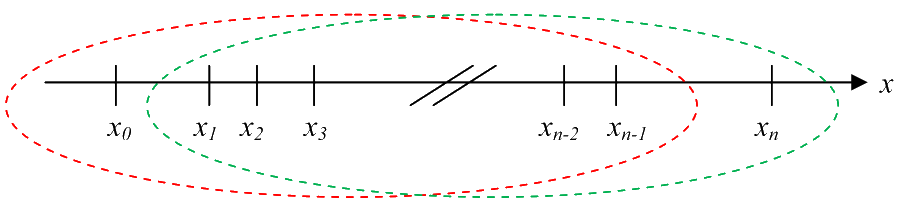
\includegraphics[width=\textwidth]{bilder/aitkenNevilleIdee}
\end{minipage}
\hfill
\begin{minipage}{11cm}
    \[
        p(x) = p_{0,1,\ldots,n}(x) = \frac{(x-x_0) \cdot \overbrace{p_{1,2,\ldots,n}}^{\text{green}}(x) - (x-x_n) \cdot \overbrace{p_{0,1,\ldots,n-1}}^{\text{red}}(x)}{(x_n - x_0)}
    \]
\end{minipage}

\subsection{Newton Polynome} \label{ssec:newton_polynom}
\textbf{Eigenschaften}
\begin{liste}
	\item[\textbf{+}] Eingebettet (Wenn ein Messwert dazukommt muss nicht alles neu berechnet werden)
	\item[\textbf{+}] Eine einzige Formel
	\item[\textbf{+}] Praktisch: Messungen sind gleichverteilt.
	\item[$\mathbf{-}$] Runge-Phänomen (Schwingungen am Rand)
	\item[$\mathbf{-}$] Aufwändig zum rechnen
\end{liste}

\begin{minipage}[t]{7.5cm}
	\begin{align}
		y_0 &= a_0\cdot \pi_0 \nonumber\\
		&\quad \downarrow\nonumber\\
		y_1 &= a_0\cdot \pi_0 +a_1\cdot\pi_1 \nonumber\\
		&\quad \downarrow \hspace{1.2cm}\downarrow\nonumber\\
		y_2 &= a_0\cdot \pi_0 +a_1\cdot\pi_1  +a_2\cdot\pi_2  \nonumber\\
		&\vdots\hspace{0.3cm}\downarrow \hspace{1.5cm}\searrow\hspace{1.5cm}\searrow\nonumber\\
		y_n &= a_0\cdot \pi_0(x_n) +a_1\cdot\pi_1(x_n)  +a_2\cdot\pi_2(x_n)+\ldots+ a_n\pi_n(x_n) \nonumber
	\end{align}

	Annäherung an ``Messreihe'' mit Polynomen: $$y(x)\approx p(x) = a_0 \pi_0(x) + a_1 \pi_1(x) + \ldots+ a_{n} \pi_{n}(x)$$
\end{minipage}
\hfill
\begin{minipage}[t]{11.5cm}
	\begin{align}
		\pi_0 &= 1 \nonumber\\
		\pi_1 &= (x-x_0) \nonumber\\
		\pi_2 &= (x-x_0)(x-x_1) \nonumber\\
		&\vdots \nonumber\\
		\pi_n &= (x-x_0)(x-x_1)\ldots(x-x_{n-1}) \nonumber\\
		\pi_{n+1} &= (x-x_0)(x-x_1)\cdots(x-x_{n-1})(x-x_n) \nonumber
	\end{align}	
\end{minipage}

\subsection{Dividierte Differenzen}
Bemerkung:
\[
	a_{p-1} = y(x_0,x_1,x_2, ... , x_p) \text{ gehört zu } \pi_{p-1}=(x-x_0)\cdot(x-x_1)\cdot ... \cdot (x-x_{p-2})
\]
Elegantere und schnellere Auflösung der Newton Polynome.
$$y(x_\mathbf{0}, x_1, \ldots x_\mathbf{k}) = \frac{y(x_\mathbf{1},x_2,\ldots x_\mathbf{k})-y(x_\mathbf{0},x_1,\ldots x_{\mathbf{k-1}})}{(x_k-x_0)} \quad (k=0,1,\ldots,n)$$
$$a(x_\mathbf{0},\ldots,x_\mathbf{n})=\frac{a(x_\mathbf{1},\ldots,x_\mathbf{n})-a(x_\mathbf{0},\ldots,x_{\mathbf{n-1}})}{x_n-x_0}$$
\begin{tabular}{ll}
$k=0$ &$y(x_0)$ \\[0.2cm]
$k=1$ &$\frac{y(x_1)-y(x_0)}{(x_1-x_0)}$\\[0.2cm]
$k=2$ &$\frac{y(x_1,x_2)-y(x_0,x_1)}{(x_2-x_0)}$\\[0.2cm]
$k=3$ &$\frac{y(x_1,x_2,x_3)-y(x_0,x_1,x_2)}{(x_3-x_0)}$\\
\end{tabular}\\
\\

\textbf{Symmetrie:} $y(x_0,x_1) = y(x_1,x_0) \Longrightarrow y(x_0,x_1,...,x_n)$ ist unabhängig von der Reihenfolge der x-Werte! (Die letze Differenz $a_n$ stimmt überein, die anderen Differenzen weichen ab.)

\paragraph{Beispiel:}~\\
\begin{minipage}[c]{6.0cm}
	\begin{tabular}{|c||c|llll|}
	\hline
			&$x_k$	&\multicolumn{4}{l|}{$y_k$}\\
	\hline
	$x_0$	&$0$	&\kreisS{$1$}{$a_0$}&			&			&\\
		 	&		&			&\kreisS{$0$}{$a_1$}&			&\\
	$x_1$	&$1$	&$1$		&			&\kreisM{$\frac 12$}{$a_2$}&\\
			&		&			&$1$		&			&\kreisB{$-\frac{1}{12}$}{$a_3$}\\
	$x_2$	&$2$	&$2$		&			&$\frac 16$&\\
			&		&			&$\frac{3}{2}$		&			&\\
	$x_3$	&$4$	&$5$		&			&			&\\
	\hline
	\end{tabular}
\end{minipage}
\hfill
\begin{minipage}[c]{13cm}
	\begin{alignat}{4}
		y(x)\approx p(x)&=a_0\cdot \pi_0(x) &&+a_1\cdot\pi_1(x)  &&+a_2\cdot\pi_2(x)&&+ a_3\pi_n(x)\nonumber\\[0.3cm]
		&=1\cdot \pi_0(x) &&+0\cdot\pi_1(x)  &&+\frac 12\cdot\pi_2(x)&&- \frac 1{12}\pi_n(x)\nonumber %\\[0.3cm]
		%&=1&&&&+\frac 12 (x-x_0)(x-x_1) &&-\frac 1{12} (x-x_0)(x-x_1)(x-x_2)\nonumber
	\end{alignat}
	\begin{alignat}{3}
	y(x)\approx p(x)&=1&&+\frac 12(x-x_0)(x-x_1)&&-\frac 1{12} (x-x_0)(x-x_1)(x-x_2)\nonumber\\[0.3cm]
	&=1&&+\frac 12(x-0)(x-1)&&-\frac 1{12} (x-0)(x-1)(x-2)\nonumber
	\end{alignat}
\end{minipage}


\subsection{Collocation Fehlerformel}
$$y(x)-p(x) = \frac{y^{(n+1)}(\xi)}{(n+1)!} (x-x_0)(x-x_1)\ldots(x-x_{n-1})(x-x_n) = \frac{y^{(n+1)}(\xi)}{(n+1)!}\pi_{n+1}(x) \quad \xi \in (\min(x_i), \max(x_i))$$

Herleitung: $y = p + \frac{y^{(n+1)}(\xi)}{(n+1)!} \cdot \pi_{n+1} = y(x_0,x_1,...,x_n) + \frac{y^{(n+1)}(\xi)}{(n+1)!} \cdot \pi_{n+1} \Longrightarrow y(x_0,x_1,...,x_{n+1}) = \frac{y^{(n+1)}(\xi)}{(n+1)!}$\\

Der Fehlerterm kann als Ableitung interpretiert werden. Es ist aber nicht klar wo die Ableitung im Bereich $[x_0,x_n]$ ausgewertet wird, da $\xi$ nicht bekannt ist!

\subsection{Runge Phänomen und Chebyshev Argumente}
\textbf{Runge Phänomen:} Potenzielle Oszillationen an den Definitionsrändern von Polynom-Collocations.
Verursacht durch hohe $n$ und hohe $\frac{y^{(n+1)}(x)}{(n+1)!}$. \\
\textbf{Chebyshev-Argumente:} Anpassung der Messpunkte durch andere Verteilung (nicht mehr gleichverteilte $x_k$, sondern am Einheitskreis gleichverteilte)
\[x_k = \cos({\frac{2k+1}{2(n+1)}\pi), \quad (k=0,1,\ldots,n)}) \]
ergibt maximale Amplitude $\max_{-1\leq x\leq 1}|\pi_{n+1}(x)| = \frac{1}{2^n}$. 
Mit affiner Transformation von Einheitsintervall $[-1,1]$ zu $[a,b]$: $x \rightarrow a+\frac{b-a}{2}(x+1)$
\begin{center}
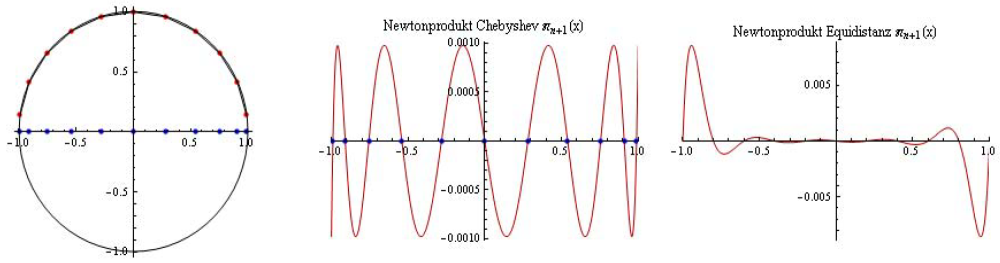
\includegraphics[width=14cm]{bilder/TschbyNewtonVergleich.png}
\end{center}

\textbf{Eigenschaften}
\begin{liste}
  \item[\textbf{+}] Kein Runge-Phänomen (Schwingungen am Rand)
  \item[\textbf{+}] Eine einzige Formel
  \item[$\mathbf{-}$] "`Nicht eingebettet"' (neue Messungen bedeutet, neue Polynomberechnung!)
  \item[$\mathbf{-}$] Praktisch: Messungen sind oft nur gleichverteilt möglich (Randauflösung beschränkt)
  \item[$\mathbf{-}$] Der Bereich der Interpolation ist fixiert (Extrapolation schlecht! (ausserhalb vom Rand))
\end{liste}


\subsection{Gleichverteilte Argumente}

\begin{minipage}[c]{11.0cm}
	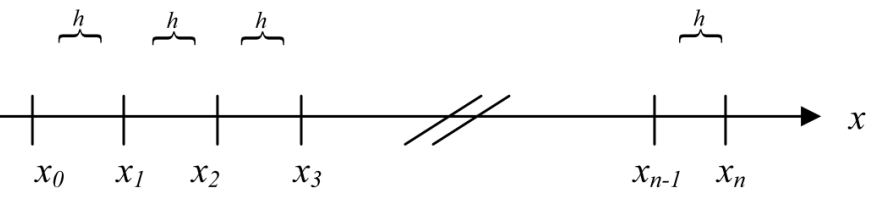
\includegraphics[width=0.8\textwidth]{bilder/gleichvArgum.png}	
\end{minipage}
\begin{minipage}[c]{6.0cm}
	$$x_k=x_0+k h\qquad k=0,1,2,\ldots n$$
	$$\boxed{y(x_0,x_1,\ldots,x_k)=\frac{\Delta^k y_0}{h^k k!}}$$
\end{minipage}
\hfill\\

$$p(x)=y_0+\frac{\Delta^1 y_0}{h^1 1!}\pi_1(x)+\frac{\Delta^2 y_0}{h^2 2!}\pi_2(x)+\ldots+\frac{\Delta^n y_0}{h^n n!}\pi_n(x)=\sum\limits_{k=0}^{n}{\frac{\Delta^k y_0}{h^k k!}\pi_k(x)}$$

\begin{center}
    \begin{tabular}{|l|lccccccccc|}
        \hline
        $\Delta^0$ && $y_0$ && $y_1$ && $y_2$ && $y_3$ && $y_4$ \\ \hline
        $\Delta^1$ &&   & $y_1-y_0$ && $y_2-y_1$ && $y_3-y_2$ && $y_4-y_3$ & \\
                   &&   & $\Delta y_0$ && $\Delta y_1$ && $\Delta y_2$ && $\Delta y_3$ & \\ \hline
        $\Delta^2$ && && $\Delta y_1-\Delta y_0$ && $\Delta y_2-\Delta y_1$ && $\Delta y_3-\Delta y_2$ && \\
                   && && $\Delta^2 y_0$ && $\Delta^2 y_1$ && $\Delta^2 y_2$ && \\ \hline
    \end{tabular}
\end{center}


\subsection{Taylor Reihe}
$$f(x)=\underset{\text{Taylor Polynom p(x)}}{\underbrace{y_0+\frac{y'(x_0)}{1!}(x-x_0)+\frac{y''(x_0)}{2!}(x-x_0)^2+\ldots+\frac{y^{(n)}(x_0)}{n!}(x-x_0)^n}}+\underset{\text{Lagrange Fehlerterm}}{\underbrace{\frac{y^{(n+1)}(\xi)}{(n+1)!}(x-x_0)^{n+1}}}$$

\section{Hermite Interpolation (Osculation)}
Erweiterung der dividierten Differenzen: Es sind jetzt auch Ableitungen an Messpunkten als 
Bedingungen möglich.
$$y(\underbrace{x_0, \ldots x_n, x_{n+1}}_{(n+2)}) = \frac{y^{(n+1)}(\xi)}{(n+1)!}$$
$$y(\underbrace{x_0, \ldots x_0}_{(n+1)}) = \lim_{\xi \rightarrow x_0} \frac{y^{(n)}(\xi)}{(n)!} = \frac{y^{n}}{\hilight{n!}}$$

Wichtig ist, dass bei der Berechnung der dividierten Differenzen keine Löcher entstehen! Dann ist das 
Gleichungssystem nicht lösbar! Es kann bei unbestimmten Resultaten eine Variable eingesetzt werden,
welche am Schluss ermittelt werden kann.
\renewcommand{\arraystretch}{1.0}
\begin{minipage}{10cm}
	\begin{tabular}{|c|lll|}
		\hline
		$x$		&\multicolumn{3}{l|}{$y$}\\
		\hline
		$x_0=2$	&$y(x_0)=1$	&							&\\
				&			&$\frac{y^{(1)}(x_0)}{1!}=1$&\\
		$x_0=2$	&$y(x_0)=1$	&							&$\frac{y^{(2)}(x_0)}{2!}=0$\\
				&			&$\frac{y^{(1)}(x_0)}{1!}=1$&\\
		$x_0=2$	&$y(x_0)=1$	&							&\\
				&			&							&\\
		$x_1=4$	&$y(x_1)=2$	&							&\\
				&			&$\frac{y^{(1)}(x_1)}{1!}=0$&\\
		$x_1=4$	&$y(x_1)=2$	&							&$\frac{y^{(2)}(x_1)}{2!}=0$\\
				&			&$\frac{y^{(1)}(x_1)}{1!}=0$&\\
		$x_1=4$	&$y(x_1)=2$	&							&\\
		\hline
	\end{tabular}
\end{minipage}
\hfill
\begin{minipage}{10cm} 
	\begin{tabular}{|c|llllll|}
		\hline
		$x$	&\multicolumn{6}{l|}{$y$}\\
		\hline
		$2$	&\kreisS{$1$}{$a_0$}&			&			&			&				&\\
			&		&\kreisS{$1$}{$a_1$}		&			&			&				&\\
		$2$	&$1$	&			&\kreisS{$0$}{$a_2$}		&			&				&\\
			&		&$1$		&			&\kreisM{$-\frac 18$}{$a_3$}&				&\\
		$2$	&$1$	&			&$-\frac 14$&			&\kreisM{$\frac 1{16}$}{$a_4$}	&\\
			&		&$\frac 12$	&			&$0$		&				&\kreisS{$0$}{$a_5$}\\
		$4$	&$2$	&			&$-\frac 14$&			&$\frac 1{16}$	&\\
			&		&$0$		&			&$\frac 18$	&				&\\
		$4$	&$2$	&			&$0$		&			&				&\\
			&		&$0$		&			&			&				&\\
		$4$	&$2$	&			&			&			&				&\\
		\hline
	\end{tabular}
\end{minipage}\\
\renewcommand{\arraystretch}{1.5}

Es werden die \textbf{modifizierten} Newton Polynome verwendet:
\begin{align}
p_2(x)	&=a_0\cdot \pi_0+a_1\cdot \pi_1+a_2\cdot \pi_2+a_3\cdot \pi_3+a_4\cdot \pi_4+a_5\cdot \pi_5\nonumber\\[0.3cm]
		&=a_0\cdot 1+a_1\cdot (x-x_0)+a_2\cdot (x-x_0)^2+a_3\cdot (x-x_0)^3+a_4\cdot (x-x_0)^3(x-x_1)+a_5\cdot (x-x_0)^3(x-x_1)^2\nonumber\\[0.3cm]
		&=1+(x-2)-\frac 18(x-2)^3+\frac 1{16} (x-2)^3(x-4)\nonumber
\end{align}

\subsection{Fehlerformel}

$$y(x)-p(x)=\frac{y^{(d)}(\xi)}{d!}(x-x_0)^{d_0}(x-x_1)^{d_1}\cdots (x-x_n)^{d_n}\qquad x,\xi \in \{\text{min } x_i,\text{min } x_i\}\quad\text{für}\quad i=0,1,\ldots,2$$
$d$ ist die total Anzahl Bedingungen und $d_i$ die Anzahl Bedingungen pro Stützstelle $x_i$.
\newpage

\subsection{Fehlende Ableitungen}

Bei fehlenden Ableitungsvorgaben werden Variablen eingesetzt und das Tableau mit diesen durchgerechnet. Am Schluss wird von hinten her auf die fehlenden Variablen geschlossen.\\

\textbf{Beispiel:}\\
Gesucht: Polynom 2. Ordnung, welches durch die Punkte $y(2)=1$ und $y(4)=1$ geht und die Ableitung $y'(4)=1$ aufweist.

\begin{minipage}[c]{6cm}
	\renewcommand{\arraystretch}{1.0}
	\begin{tabular}{|c|llll|}
		\hline
		$x$	&\multicolumn{4}{l|}{$y$}\\
		\hline
		$2$	&\kreisS{$1$}{$a_0$}&	&&\\
			&	&\kreisS{$\beta$}{$a_1$}&&\\
		$2$	&$1$&	&\kreisB{$-\frac \beta2$}{$a_2$}&\\
			&	&$0$&				  &\kreisB{$\frac{1+\beta}{4}$}{$a_3$}$\overset{!}{=}0$\\
		$4$	&$1$&	&$\frac 12$&\\
			&	&$1$&&\\
		$4$	&$1$&	&&\\		
		\hline
	\end{tabular}
	\renewcommand{\arraystretch}{1.5}
\end{minipage}
\hfill
\begin{minipage}[c]{12cm}

	\vspace{0.5cm}
	
	\begin{itemize}
		\item Weil das Polynom die Ordnung $d=2$ aufweisen muss, gilt: $\frac{1+\beta}4=0$\\
		Daraus folgt: $\beta=-1$
		\item Das Lösungspolynom ist:
		\begin{align} p(x)&=a_0+a_1(x-x_0)+a_2(x-x_0)^2+a_3(x-x_0)^2(x-x_1)\nonumber\\
		&=1+\beta(x-x_0)-\frac \beta2(x-x_0)^2+\frac{1+\beta}4(x-x_0)^2(x-x_1)\big|_{\beta=-1}\nonumber\\
		&=1-(x-2)+\frac 12(x-2)^2\nonumber
		\end{align}
	\end{itemize}
\end{minipage}

\vfill

\section{Multi-variate Polynomial Interpolation}
\begin{tabular}{ll}
  \parbox{6cm}{
    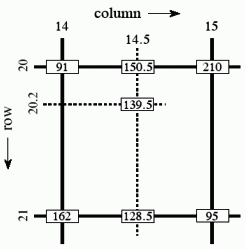
\includegraphics[width=6cm]{./bilder/bilineare_interpolation}
  }
  & \parbox{12.5cm} {
    \begin{aufzaehlung}
      \item 
        Die Basis der Polynome kann durch das \emph{2-fold tensor product} berechnet werden $\Rightarrow$ Bilineare Interpolation \\
        $\{1,x,x^2\} \otimes \{1, y, y^2\} = \{1,x,y,x^2,y^2,xy, x^2y, xy^2, x^2y^2\}$; \\
        Dadurch kann die Anzahl Gleichungen n berechnet werden: \\$\mathbb R^n \otimes \mathbb R^k = \mathbb R^{nk}$
      \item Interpolation der gewünschten Ordnung (linear, quadratisch, \ldots) in X-Richtung an 
        Stelle $y_0$ berechnen: $p(x,y_0)$
      \item Interpolation der gewünschten Ordnung (linear, quadratisch, \ldots) in X-Richtung an 
        Stelle $y_1$ berechnen: $p(x,y_1)$
      \item Tableau für dividierte Differenzen berechnen (hier linearer Fall):\\
        \begin{tabular}{l|ll}
          $y$ & $z$\\
          \hline
          $y_0$ & $p(x,y_0) = a_{y0}$\\
          $y_1$ & $p(x,y_1)$ & $\frac{p(x,y_1) - p(x,y_0)}{y_1-y_0} = a_{y1}$
        \end{tabular}
      \item Polynom aufstellen:\\
        $p(x,y) = a_{y0} \pi_0(y) + a_{y1} \pi_1(y) + a_{y2} \pi_2(y)+\ldots$
      \item Polynom ausmultiplizieren:\\
          $p(x,y) = a_{0,0} \pi_0(x)\pi_0(y) + a_{1,0} \pi_1(x)\pi_0(y) + a_{0,1} \pi_0(x)\pi_1(y) + a_{1,1} \pi_1(x)\pi_1(y)+\ldots$ 
    \end{aufzaehlung}
  }

\end{tabular}
\subsection{Beispiel:}
Die Punkte $(14,20),(14,21),(15,20)(15,21)$ sind gegeben: $\{91/255, 162/255, 210/255, 95/255\}$. Gesucht ist eine lineare interpolation. 
Das ergibt folgende Polynom Basen: $(\{1,x\}\times\{1,y\}=\{1,x,y,xy\})$\\
\begin{enumerate}
  \item Interpolation für $y=y_0=20$: $p(x,y_0)= p(x_0,y_0) \pi_0(x) + \frac{p(x_1,y_0)-p(x_0,y_0)}{x_1-x_0}\pi_1(x)=\frac{1}{255}\left(91 \cdot 1 + \frac{210-91}{15-14}\cdot(x-14)\right)$
  \item Das selbe für $y=y_1=21$:  $p(x,y_1)=\frac{1}{255}\left(162 \cdot 1 + \frac{95-162}{15-14}\cdot(x-14)\right)$
  \item Dann die schlussendliche Interpolation: $p(x,y)=p(x,y_0)\pi_0(y)+\frac{p(x,y_1)-p(x,y_0)}{y_1-y_0}\pi_1(y)$\\
  $=\frac 1{255} \left((91\cdot 1 +\frac{210-91}{15-14}\cdot 1)\cdot 1 + \frac{162\cdot 1 \frac{95-162}{15-14}\cdot (x-14)-91\cdot 1 + \frac{210-91}{15-14}\cdot(x-14)}{21-20}\cdot(y-20)\right)
  =-215.98 + 15.0549 x + 10.4902 y - 0.7294 x y$
\end{enumerate}

%TODO: bi-cubic und multivariate
\clearpage
\section{Spline-Interpolation}

\begin{minipage}[c]{14.5cm}
Die Idee der Spline-Interpolation ist, die Daten nicht mit einem Polynom hohen Grades zu interpolieren, sondern mit mehreren Polynomen tiefen Grades. Daduch kann die Tendenz  zum Schwingen von Polynomen hohen Grades umgangen werden. Bei den "Bruchstellen", den Übergängen von einem Patch zum nächsten, müssen die Ableitungen der benachbarten Patches bis zu einem vorgegeben Ableitung übereinstimmten.
\end{minipage}
\hfill
\begin{minipage}[c]{4cm}
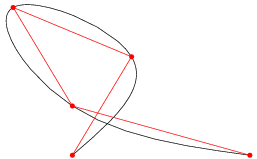
\includegraphics[width=\textwidth]{bilder/kubikSpline}
\end{minipage}

\textbf{Eigenschaften}
\begin{liste}
  \item[\textbf{+}] Kein Runge-Phänomen (Schwingungen am Rand)
  \item[\textbf{+}] Polynome haben tiefen Grad
  \item[\textbf{+}] Aufwand zur Berechnung geringer als Newton [Spline: $O(n)$ (wegen Tridiagonaler Band-Matrix), Newton: $O(n^2)$]  
  \item[$\mathbf{-}$] "`Nicht eingebettet"' (neue Messungen bedeutet, neue Polynomberechnung!)
  \item[$\mathbf{-}$] Polynome müssen zur Auswertung zusammengesetzt werden (Post-Processing Aufwand gross)
\end{liste}


\subsection{Ein-Dimensionale Splines}
\subsubsection{Prinzip}
Pro \em Patch \em (von total $n$) wird ein Polynom vom Grad $d$ (meist kubisch, $d=3$) berechnet. An den Übergängen 
bei $x_i$ können Bedingungen $C^k$ ($k=1,\ldots, d-1$) definiert werden.

\paragraph{Freiheitsgrade}
$n$ Patches mit je 1 Polynom mit je $(d+1)$ Koeffizienten, gibt total $n(d+1)$ Freiheitsgrade.

\paragraph{Bedingungen}
$n$ Patches mit Anfang und Ende $=2n$;
$d-1$ Ableitungen pro innerem Punkt $(n-1)(d-1)$ ergibt total ($(n(d+1)-(d-1))$) Bedingungen.

\paragraph{Zusatzbedingungen}

Vergleicht man Freiheitsgrade und Bedinungen, sind $d-1$ Bedingungen zu wählen. Beim \em natural 
spline \em werden dazu die zweiten Ableitungen auf 0 gesetzt; beim \em clamped splines \em werden
die 1. Ableitungen vorgegeben.


\subsubsection{Allgemeines Vorgehen (kubische Splines)}
Die endgültige Interpolation hat folgende Form (Beschreibung \textbf{eines} Patches):
$$\boxed{S_i(x) = a_i + b_i(x-x_i) + c_i(x-x_i)^2 + d_i(x-x_i)^3}$$
$$S_i' = b_i + 2c_i(x-x_i)+3d_i(x-x_i)^2$$
$$S_i'' = 2c_i + 6 d_i (x-x_i)$$
Gebraucht wird auch (Patch-Breite) $h_i = x_{i+1} - x_i = \Delta x_i$ 
\begin{enumerate}
  \item $a_i = y_i \qquad (i=0,\ldots n-1)$
  \item Für kubische Splines hat es $d-1=3-1=2$ Zusatzbedingungen.\\ 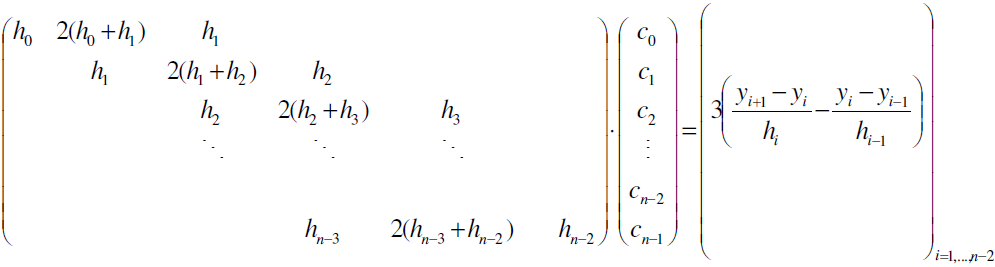
\includegraphics[width=12cm]{./bilder/1d_spline_gleichungssystem}
\newpage
    \begin{itemize}
      \item \textbf{Natural Splining} (Randkrümmung): $y_0''=0=y_n''$ (minimiert das Energiemass! ($\min \int |f''(x)|^2 \mathrm{d}x$))
        \begin{enumerate}
          \item $c_0 = c_n = 0$
          \item Gleichungssystem nach $c_i$ auflösen:\\
            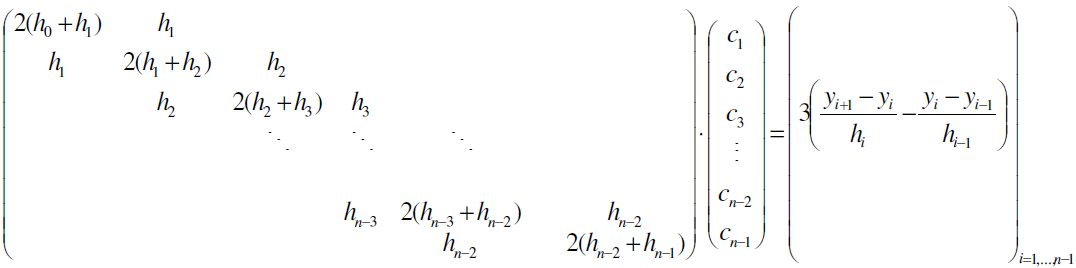
\includegraphics[width=13cm]{./bilder/1d_spline_natural_gleichungssystem}
          %\item $d_{n-1} = -\frac{c_{n-1}}{3h_{n-1}}$
        \end{enumerate}        
       \item \textbf{Clamped Splining:}
         \begin{enumerate}
           \item $b_0 = y_0'; b_n=y_n'$
           \item Gleichungssystem nach $c_i$ auflösen:\\
             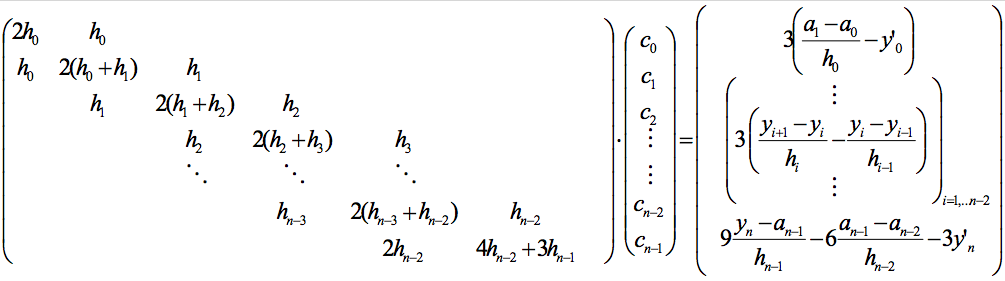
\includegraphics[width=12cm]{./bilder/ClampedSplining}
           %\item $d_{n-1} = \frac{y_n' - b_{n-1} - 2c_{n-1}h_{n-1}}{3h_{n-1}^2}$ (am Schluss zu berechnen)
         \end{enumerate}
    \end{itemize}
  \item $b_{i-1} = \frac{a_i - a_{i-1}}{h_{i-1}} - \frac{2 c_{i-1} + c_i}{3} h_{i-1} \qquad (i=1, \ldots n-1)$
  \item $b_{n-1} = \frac{y_n - a_{n-1}}{h_{n-1}} - c_{n-1} h_{n-1} - d_{n-1}h_{n-1}^2=\frac{y_n-y_{n-1}}{h_{n-1}}-\frac 23 c_{n-1}h_{n-1}$
  \item $d_{i-1} = \frac{c_i - c_{i-1}}{3 h_{i-1}} \qquad (i=1, \ldots n-1)$
  \item Clamped splining: $d_{n-1} = \frac{y_n' - b_{n-1} - 2c_{n-1}h_{n-1}}{3h_{n-1}^2}$ \hspace{1cm} Natural Splining: $d_{n-1} = -\frac{c_{n-1}}{3h_{n-1}}$
\end{enumerate}

\paragraph{Weitere Methoden}~\\
Bei \emph{Hermite cubic splines} werden $C^1$-Funktionen aus gepatchten kubischen Polynomen mit
vorgegebenen ersten Ableitungen gebildet.

\emph{Periodic splines} sind $C^2$ Funktionen aus gepatchten kubischen Polynomen mit Periodizität ($S'(x_0)=S'(x_n)$ und $S''(x_0)=S''(x_n)$).

\subsubsection{Fehlerabschätzung}
Für kubische Splines mit $C^2$ gilt folgende Fehlerabschätzung ($H = \max h_i \; (i=0, \ldots n-1)$):\\
$| y(x) - S(x) | \leq \max |y^{(4)}(x)| \frac{5}{384} H^4 \qquad
 | y'(x) - S'(x) | \leq \max |y^{(4)}(x)| \frac{1}{24} H^3 \qquad 
 | y''(x) - S''(x) | \leq \max |y^{(4)}(x)| \frac{3}{8} H^2$
 
 
\newpage
\subsection{Bernstein-Bézier Splines (B-B Splines)}

\begin{minipage}[c]{15.0cm}	
	\subsubsection{Bernstein-Polynome}
    	Die Bernstein-Polynome sind im Intervall $t\in[0,1]$ definiert als
	    \[B_{i,n}(t) = \binom{n}{i}(1-t)^{n-i} t^i \qquad t \in [0,1]\; i=0,1,\ldots, n\]
	    mit $i$: Nr und  $n$: Ordnung des Splines.
	    
        Mittels einer affinen Transformation in den Bereich $t \in [a,b]$ folgt	    
	    \[B_{i,n}(u,a,b) =\frac{1}{(b-a)^n}\binom{n}{i}(b-u)^{n-i} (u-a)^i \qquad u \in [a,b]\; i=0,1,\ldots, n\]
	    
	\paragraph{Eigenschaften}
		Bernstein Polynome$\ldots$
	    \begin{itemize}
	      \item ergeben eine lineare Basis für Polynome der Ordnung $n$ (man kann mit ihnen jedes Polynom der Ordnung $n$ zusammenbauen)
	      \item haben genau eine Maximalstelle bei $t=\frac in$
	      \item haben eine Nullstelle bei $0$ (Ordnung $i$) und bei $1$ (Ordnung $n-1$)
	      \item sind symmetrisch: $B_{i,n}(t) = B_{n-i,n}(1-t)$
	      \item sind zwischen $t \in [0,1]$ begrenzt auf $[0,1]$
	      \item ergeben in der Summe: $\sum \limits_{i=0}^n B_{i,n}(t)=1$
	    \end{itemize}
	    
	    $\frac{d}{dt} B_{i,n}(t) = n(B_{i-1,n-1}(t) - B_{i,n-1}(t)) = -n \Delta B_{i-1,n-1}(t)$\\
	    $\frac{d^2}{dt^2} B_{i,n}(t) = n(n-1)(B_{i-2,n-2}(t) -2 B_{i-1,n-2}(t) + B_{i,n-2}(t)) = n(n-1) \Delta^2 B_{i-2,n-2}(t)$\\
	    $\frac{d^k}{dt^k} B_{i,n}(t) = (-1)^k n(n-1)\ldots(n-k+1) \Delta^k B_{i-k,n-k}(t)$
\end{minipage}
\hfill    
\begin{minipage}[c]{4cm}
  	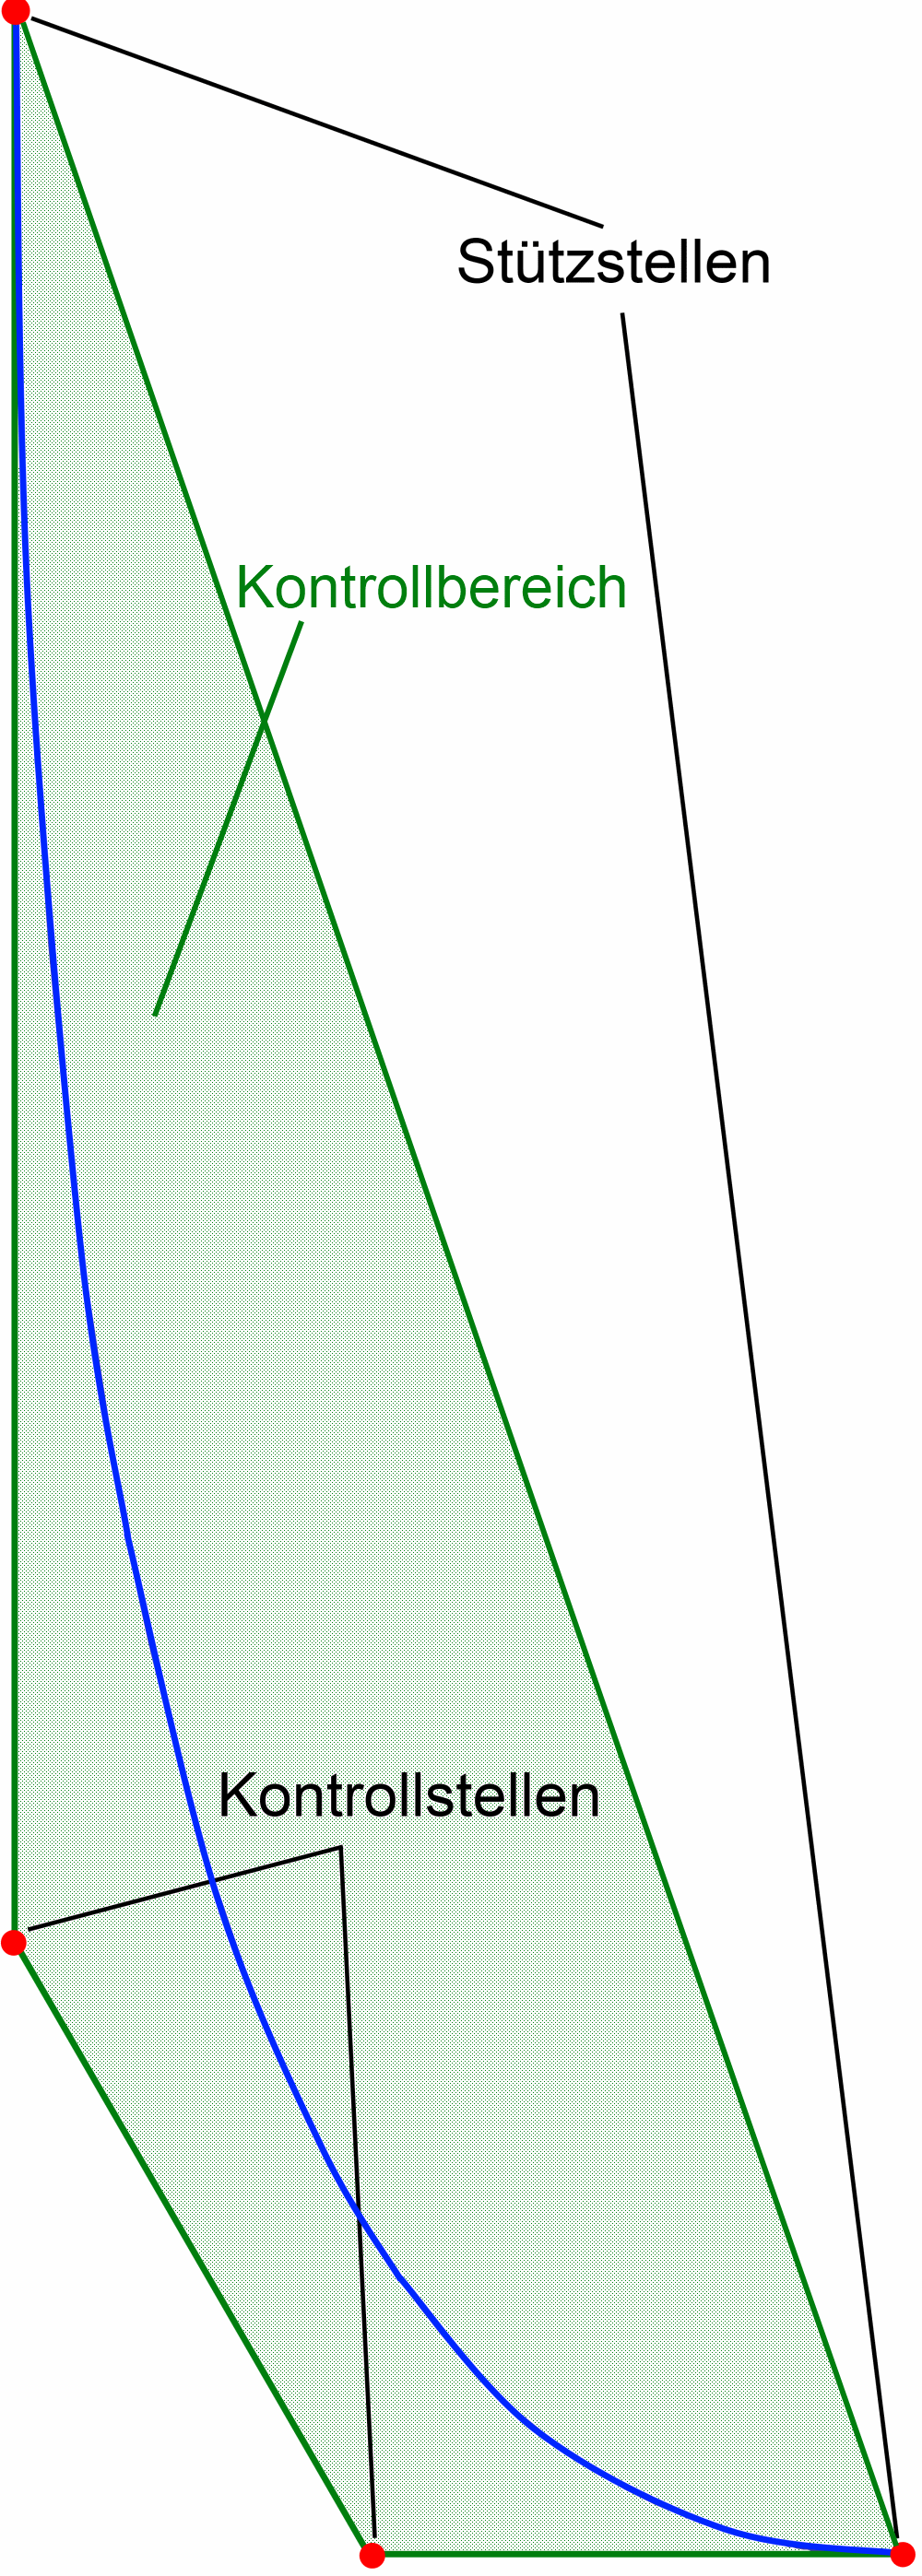
\includegraphics[width=\textwidth]{bilder/bernsteinBezier}
\end{minipage}

\vspace{0.2cm}

\begin{minipage}[c]{5.5cm}	
\textbf{Pascal'sches Dreieck}\\

	\scalebox{0.8}{
	\renewcommand{\arraystretch}{1}
	\begin{tabular}{rccccccccc}
		$n=0$:&    &    &    &    &  1\\\noalign{\smallskip\smallskip}
		$n=1$:&    &    &    &  1 &    &  1\\\noalign{\smallskip\smallskip}
		$n=2$:&    &    &  1 &    &  2 &    &  1\\\noalign{\smallskip\smallskip}
		$n=3$:&    &  1 &    &  3 &    &  3 &    &  1\\\noalign{\smallskip\smallskip}
		$n=4$:&  1 &    &  4 &    &  6 &    &  4 &    &  1\\\noalign{\smallskip\smallskip}
	\end{tabular}}
\end{minipage}
\hfill    
\begin{minipage}[c]{13.25cm}   
\textbf{Bernstein Polynome} \quad $0\leq t\leq 1$\\

	\scalebox{0.8}{
	\begin{tabular}{lllll}
		$B_{0,0}(t)=1$&&&&\\
		$B_{0,1}(t)=1-t$&$B_{1,1}(t)=t$&&&\\
		$B_{0,2}(t)=(1-t)^2$&$B_{1,2}(t)=2t(1-t)$&$B_{2,2}(t)=t^2$&&\\
		$B_{0,3}(t)=(1-t)^3$&$B_{1,3}(t)=3t(1-t)^2$&$B_{2,3}(t)=3t^2(1-t)$&$B_{3,3}(t)=t^3$&\\
		$B_{0,4}(t)=(1-t)^4$&$B_{1,4}(t)=4t(1-t)^3$&$B_{2,4}(t)=6t^2(1-t)^2$&$B_{3,4}(t)=4t^3(1-t)$&$B_{4,4}(t)=t^4$\\
	\end{tabular}}
\renewcommand{\arraystretch}{1.5} 
\end{minipage}  


\subsubsection{Simple Bézier Kurven}
Eine Bézier-Kurve wird über Kontrollpunkte ($\vec{P}_0, \vec{P}_1, \ldots \vec{P}_n\,(n \geq 2)$ 
in $R^d$) sowie die Bernstein Polynome definiert:
$$\vec{r}(t) = \sum \limits_{i=0}^{n} \vec{P}_i B_{i,n}(t) \quad t \in [0,1]$$
\paragraph{Eigenschaften}
\begin{itemize}
  \item Die Bézier-Kurven liegen immer innerhalb der konvexen Hülle der Kontrollpunkte.
  \item \begin{tabular}{ll}
            $\vec{r}(0) = \vec{P}_0$ & $\vec{r}(1) = \vec{P}_n$ \\
            $\vec{r}\,'(0) = n(\vec{P}_1-\vec{P}_0)$ & $\vec{r}\,'(1) = n(\vec{P}_n-\vec{P}_{n-1})$ \\
            $\vec{r}\,''(0) = n(n-1)(\vec{P}_2 - 2\vec{P}_1 + \vec{P}_0)$ & $\vec{r}\,''(1) = n(n-1)(\vec{P}_n - 2\vec{P}_{n-1} + \vec{P}_{n-2})$ \\
        \end{tabular}
  \item Wenn $C^k$ Übergang zu einem Punkt gefordert ist, sind $k$ Gleichungen bzw. $k$ 
        Kontrollpunkte pro Punkt nötig
\end{itemize}

\begin{minipage}{13.5cm}
\subsubsection{Casteljau recurrence}
Die Castaljau recurrence ist eine ähnliche Idee wie Neville-Aitken. 
Damit kann ein Punkt auf einer Bézier Kurve als Linearkombination zweier Punkte aus Bézier Kurven tieferer Ordnung berechnet werden.
\[
    \vec{r}_{\vec{P_0},\vec{P_1},\ldots,\vec{P_n}}(t) = (1-t)\cdot\vec{r}_{\vec{P_0},\vec{P_1},\ldots,\vec{P_{n-1}}}(t) + t \cdot \vec{r}_{\vec{P_1},\vec{P_2},\ldots,\vec{P_n}}(t) \qquad t \in [0,1]
\]


  \subsubsection{Zusammengesetzte (Composite) Bézier Kurven}
  Die zusammengesetzten (simplen) Bézier-Kurven sollen die bekannte Bedingungen ($C^k$) erfüllen.
  Dies sind die Gleichungen um den Punkt $Q_0$ mit Kontrollpunkten $Q_{1,\ldots,m-1}$ nach $Q_0$ sowie
  den Kontrollpunkten $P_{1,\ldots,n-1}$ vor $Q_0$. 
\end{minipage}
\begin{minipage}{5.5cm}
  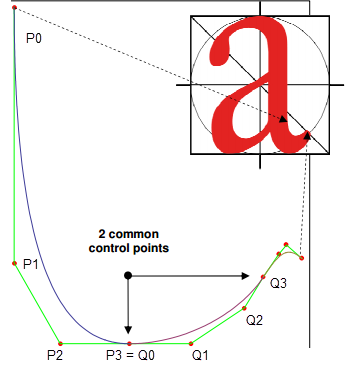
\includegraphics[width=5.5cm]{./bilder/composite_bezier.png}
  Hier sind $m=n=3$
\end{minipage}

  \begin{align*}
      &C^0: \qquad && &&\boxed{\vec{P_n} = \vec{Q_0}} \\
      &C^1: && \vec{r}\,'_P(1) = &&\boxed{n(\vec{P}_n-\vec{P}_{n-1}) = m(\vec{Q}_1-\vec{Q_0})} && = \vec{r}\,'_Q(0) \\
      &C^2: && \vec{r}\,''_P(1) = &&\boxed{n(n-1)(\vec{P}_n - 2\vec{P}_{n-1} + \vec{P}_{n-2}) = 
    m(m-1)(\vec{Q}_2 - 2\vec{Q_1} + \vec{Q_0})} && = \vec{r}\,''_Q(0) \\
      &C^k: && \vec{r}_P^{\,(j)}(1) = && \boxed{n(n-1)\dots(n-j+1)(\Delta^j\vec{P}_{n-j}) = 
      m(m-1)\dots(m-j+1)(\Delta^j\vec{Q}_0)} &&= \vec{r}_Q^{\,(j)}(0)
  \end{align*}
  
  $m$ ist dabei der Grad von $\vec{r}_Q$, $n$ derjenige von $\vec{r}_P$.
  
\subsubsection{Bézier Oberflächen als Tensor Splines}
Bézier Oberflächen werden gleich wie Bézier Kurven mittels einem Tensorprodukt aus Bernstein Polynomen gebildet.
Eine Oberfläche im Intervall $[0,1]\times[0,1]$ wird gebildet durch
\[
    \vec{z}(s,t) = \sum\limits_{i=0}^n\sum\limits_{j=0}^m \vec{P}_{ij} B_{in}(s) B_{jm}(t) \qquad s,t\in[0,1]
\]

Details und Formeln siehe Skript S. 19 -- 23.

\subsubsection{Vergleich Bézier- und Newton-Interpolation mit gleichverteilten Argumenten auf X-Achse}
  Aus Sicht Bézier:
  \begin{liste}
    \item[+] Kleiner Fehler, keine Oszillation, kein Runge (bei kleinem Grad, z.B. 3)
    \item[+] $O(n)$ (linearer Rechenaufwand)
    \item[-] Nicht eingebettet (neue Daten brauchen Neuberechnung der Interpolation)
    \item[-] Post-Processing (Grafik, Integrations, Ableitungen) sind komplexer, da jedes Kurvenstück
      einzeln betrachtet werden muss.
  \end{liste}

\newpage
\section{Least-Squares Approximation}
\subsection{Lineare Least-Squares}
Ziel: Approximation von Messpunkten durch Minimieren einer Funktion, die die Abweichung in $y$ 
angibt (Residuen). Die Datenpunkte werden bei dieser Methode nicht mehr genau getroffen, ausserdem ist der Grad $m$ des Approximation-Polynoms meist massiv kleiner als die Anzahl der gegebenen Datenpunkte $N+1$.\\

Aus einer Menge von Basisfunktionen ${g_0,g_1,\ldots,g_m}$ mit $m \ll N$ und den Messungen $(x_0,y_0),(x_1,y_1),\ldots,(x_N,y_N)$ wird das überdeterminierte ($m<N$) Gleichungssystem aufgestellt und nach den unbekannten $a_i$ gelöst.
\[
    \overbrace{
    \begin{pmatrix}
        g_0(x_0) & g_1(x_1) & \ldots & g_m(x_0) \\
        \vdots & \vdots & \ddots & \vdots \\
        \vdots & \vdots & \ddots & \vdots \\
        g_0(x_N) & g_1(x_N) & \ldots & g_m(x_N) 
    \end{pmatrix}}^{\text{Designmatrix } G}
    \cdot
    \begin{pmatrix}
        a_0 \\ \vdots \\ a_m
    \end{pmatrix}
    =
    \begin{pmatrix}
        y_0 \\ \vdots \\ \vdots \\ y_N
    \end{pmatrix}
    \qquad
    \Leftrightarrow
    \qquad
    G \cdot a = y
\]


\begin{minipage}[c]{12.5cm}
	\begin{tabular}{ll}
		Zu minimierende Fehlerfunktion:
		&$\boxed{\underbrace{S}_{Fehler}=\sum\limits_{i=0}^{N}{\big(y_i - \underbrace{\sum\limits_{j=0}^{m}{a_j g_j}}_{Modell}\big)^2} = \sum\limits_{i=0}^{N}{ r_i^2}}$\\
		Modellfunktion: 
		&$\boxed{y=\sum\limits_{j=0}^{m}{a_j g_j}}\overset{Poly!}{=}\sum\limits_{j=0}^{m}{a_j x^j}$\\
		Abweichungen (Residuen): 
		&$r_i=y_i-\sum\limits_{j=0}^{m}{a_j g_j}$
	\end{tabular}
	
	\subsubsection{Normalgleichung}
	
	Minimieren des quadratischen Fehlers mit "`Normalmatrix"' G (Designmatrix):
	$$\underbrace{\bm{G}^T \bm{G}}_{Normalmatrix}\cdot \bm{a} = \bm{G}^T \bm{y} \qquad \Rightarrow \qquad \bm{a}=(\bm{G}^T \bm{G})^{-1}\bm{G}^T \bm{y}$$
	$$\underbrace{\underbrace{\bm{G}^T}_{(m+1)\times(N+1)} \cdot \underbrace{\bm{G}}_{(N+1)\times(m+1)}}_{(m+1)\times(m+1)}\cdot
	  \underbrace{\bm{a}}_{(m+1)\times 1}=
	  \underbrace{\underbrace{\bm{G}^T}_{(m+1)\times(N+1)}\cdot\underbrace{\bm{y}}_{(N+1)\times 1}}_{(m+1)\times 1}$$
\end{minipage}
\hfill
\begin{minipage}[c]{6.5cm}
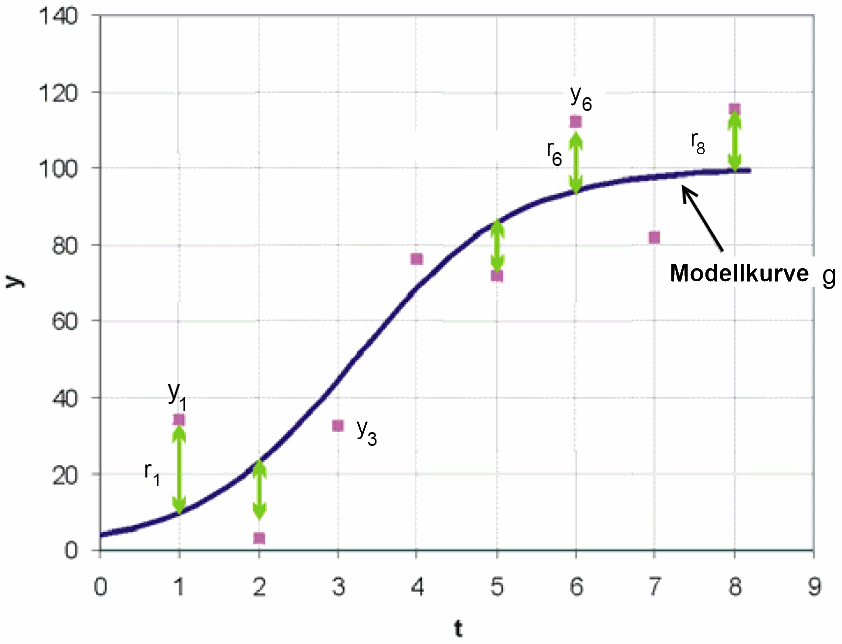
\includegraphics[width=\textwidth]{bilder/leastSquare}\\

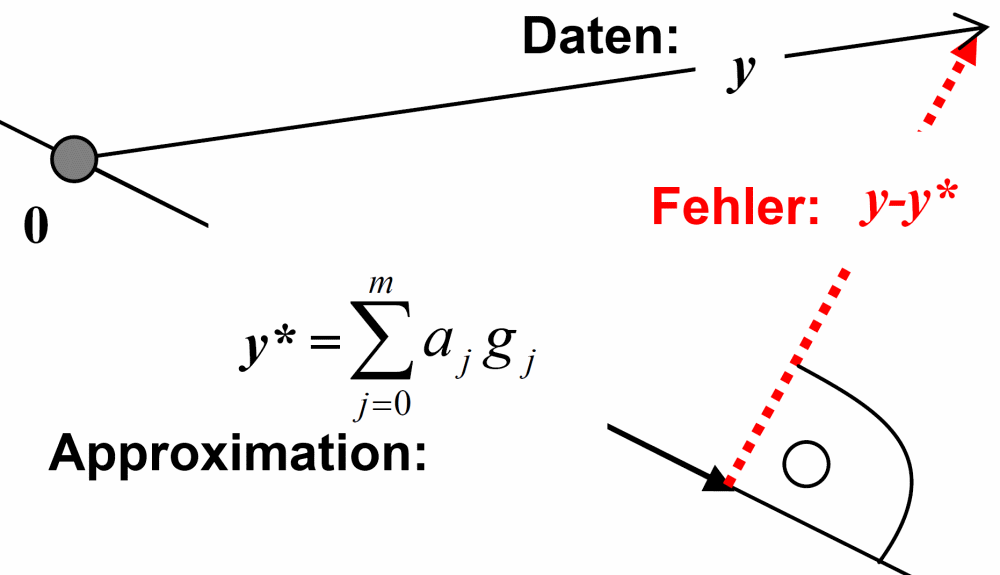
\includegraphics[width=1\textwidth,trim=-3cm 0cm 0cm 0cm]{bilder/leastSquareOrth}
\end{minipage}

Die symmetrische $(m+1)\times(m+1)$ Matrix $G^T \cdot G$ ist positiv definit wenn $g_i$ linear unabhängig sind.
Das neue Gleichungssystem ist regulär und hat eine eindeutige Lösung für die Koeffizienten $a_j$.
\[
    \overbrace{
    \begin{pmatrix}
        \langle g_0|,g_0|\rangle & \langle g_1|,g_0|\rangle & \ldots & \langle g_m|,g_0|\rangle \\
        \vdots & \vdots & ddots & \vdots \\
        \langle g_0|,g_m|\rangle & \langle g_1|,g_m|\rangle & \ldots & \langle g_m|,g_m|\rangle
    \end{pmatrix}
    }^{G^T \cdot G}
    \cdot
    \begin{pmatrix}
        a_0 \\ \vdots \\ a_m
    \end{pmatrix}
    =
    \begin{pmatrix}
        \langle y|,g_0 |\rangle \\ \vdots \\ \vdots \\ \langle y|,g_m| \rangle
    \end{pmatrix}
\]

\subsubsection{QR-Zerlegung}
Eine quadratische $n \times n$ Matrix $Q$ ist orthogonal, falls $Q^T \cdot Q = Q \cdot Q^T = I$ bzw. $Q^T = Q^{-1}$.
Jede beliebige Matrix $G$ mit den Dimensionen $(N+1) \times (m+1)$ mit $N \geq m$ und Rang $m+1$ kann als
Produkt einer orthogonalen $(N+1)\times(N+1)$ Matrix $Q$ und einer $(N+1)\times(m+1)$ oberen Dreiecksmatrix $R$.

Aus dem Gleichungssystem $Ga| = y|$ wird dann $Ra|=Q^Ty|$, was einfacher lösbar ist\textsuperscript{Citation needed}.

\subsubsection{Singulärwertzerlegung (singular value decomposition, SVD)}
Jede Matrix $\bm G$ mit Dimensionen $(N+1) \times (m+1)$ kann so zerlegt werden:
$$\bm G = \bm U \bm D \bm V^T = \bm U \cdot \begin{bmatrix}
  d_{00} & 0      & \ldots & 0\\
  0      & d_{11} & \ldots & 0\\
  \vdots & \vdots & \ddots & 0\\
  0      & \ldots & 0      & d_{mm}\\
  0      & 0      & \ldots & 0\\
  \vdots & \vdots & \ddots & 0\\
  0      & 0      & \ldots & 0
\end{bmatrix} \cdot \bm V^T$$
$\bm D$ ($(N+1) \times (m+1)$) ist die zentrale Diagonalmatrix mit Singulärwerten,
$\bm U$ ($(N+1) \times (N+1)$) und $\bm V$ ($(m+1) \times (m+1)$) sind orthogonale und quadratische
Matrizen (d.h. u.a. $\bm U^T=\bm U^{-1}$).\\

Die Zerlegung an sich wird hier nicht weiter ausgeführt, diese kann anderswo nachgeschlagen werden.
SVD kann gebraucht werden, um Gleichungssystem zu lösen (wie hier), um Eigenvektoren und Eigenwerte 
sowie die Inverse zu berechnen.

Aus $Ga|=y|$ wird $UDV^T a|=y|$. Dies lässt sich auflösen zu
\[
    a| = V D^{-1}U^T \cdot y|
\]

\subsubsection{Monomiale} \label{sssec:ls_monomiale}
Mit 
$g = a_0 \underbrace{1}_{g_0} + a_1 \underbrace{x}_{g_1} + a_2 \underbrace{x^2}_{g_2} +\ldots + a_m \underbrace{x^m}_{g_2}$ 
wird die Designmatrix zu:
\[G \underbrace{=}_{\text{When Monomials}} 
\begin{bmatrix}
  1 & x_0 & x_0^2  & \ldots & x_0^m\\
  1 & x_1 & x_1^2  & \ldots & x_1^m\\
  \vdots  & \vdots & \vdots  & \ddots & \vdots\\
  1 & x_N & x_N^2  & \ldots & x_N^m\\
\end{bmatrix}\]


\subsubsection{Gleichförmige Argumente\quad (Orthogonalitäts-Eigenschaften)} \label{sssec:ls_orthogonal}
Mit gleichförmigen Elementen $x_i - x_j = (j-i) h$ für alle $i,j$ $\rightarrow$ $\{x_0...x_N\} = \{x_0 + t \cdot h\}_{t=0...N}$ und \textbf{orthogonalen Polynomen} kann 
$G G^T$ diagonalisiert und so die Gleichungen rechnerisch einfacher gelöst werden. 

$$\boxed{p_{k,N}(t) = \sum_{i=0}^k (-1)^i \binom{k}{i} \binom{k+i}{i} \frac{t^{(i)}}{N^{(i)}}= 
1+\sum_{i=1}^k (-1)^i \binom{k}{i} \binom{k+i}{i} \frac{t(t-1)(t-2)\ldots(t-i+1)}{N(N-1)(N-2)\ldots(N-i+1)} \qquad (k = 1,\ldots,N)}$$
mit $t=\frac{x-x_0}{h} \qquad \binom{k}{i}=\frac{k!}{i!(k-i)!}=nCr(k,i)$\\
$p_{k,N}$ kann jetzt als $g_{k}$ in die Designmatrix eingesetzt werden und das Produkt $G^T G$ wird 
zu einer $(m+1)\times(m+1)$ Diagonalmatrix. Schlussendlich kann $a$ über die bekannte Formel
$G^T G a = G^T y$ berechnet werden.\\

\textbf{Beispiel:}
$$\bm{x}=
	   \begin{bmatrix}
			3&4&5&6&7
	   \end{bmatrix}\qquad \Rightarrow\qquad \bm{t}=\bm{x}-3=
	   \begin{bmatrix}
	   		0&1&2&3&4
	   \end{bmatrix}$$
$$\Rightarrow P_0(x)=1 \qquad P_1(x)= 1-\frac{x-3}{2}\qquad P_2(x)=1-\frac{2\cdot 3 (x-3)}{4}+\frac{1 \cdot 3 (x-3)(x-3 -1)}{4 \cdot 3} = 1-\frac{3x-9}{2}+\frac 12 (x-4)(x-3)???$$
$$\overset{\hspace{0.6cm} P_0 \hspace{0.5cm} P_1 \hspace{0.6cm} P_2}{\bm{G} = \begin{bmatrix}
  1 & 1 	& 1\\
  1 & 1/2 	& -1/2\\
  1 & 0	  	& -1\\
  1 & -1/2 	& -1/2\\
  1 & -1 	& 1\\
\end{bmatrix}}\qquad \Rightarrow\qquad
\bm{G}^T\bm{G}=\begin{bmatrix}
 \| P_0\|^2 	& 0 	& 0\\
  0 		& \|P_1\|^2 	& 0\\
  0 		& 0	  	&\|P_2\|^2\\
\end{bmatrix}
= \begin{bmatrix}
  5 & 0 & 0 \\
  0 & \frac52 & 0\\
  0 & 0 & \frac{7} {2}\\
\end{bmatrix}
$$

\newpage
\subsubsection{Chebyshev Orthogonale Polynome} \label{sssec:chebyshev_polynom}
\textbf{Idee}: Approximation eines kontinuierlichen Polynoms durch Chebyshev-Polynome.

\textbf{Definition}\\
Chebyshev Polynome sind definiert als $\boxed{T_n(x) = \cos(n \arccos(x))}$ mit $(n = 0,1,\ldots)$ und $(-1 \leq x \leq 1)$. Dieses 
Polynom bewirkt eine Häufung der Messwerte in den Randbereichen. Die
ersten paar Polynome $T_n$ sowie deren Umformungen nach $x$:\\
\begin{tabular}{ll}
  $T_0 = 1$ & $x^0 = 1 = T_0$ \\
  $T_1 = x$ & $x^1 = x = T_1$ \\
  $T_2 = 2x^2 -1$ & $x^2 = \frac12 T_2 + \frac12 T_0$ \\
  $T_3 = 4x^3 - 3x$ & $x^3 = \frac14 T_3 + \frac34 T_1$\\
  $T_4 = 8x^4 -8x^2 + 1$ & $x^4 = \frac18 T_4 + \frac12 T_2 + \frac38 T_0$\\
  $T_5 = 16x^5 - 20x^3 + 5x$ & $x^5 = \frac{1}{16} T_5 + \frac{5}{16} T_3 + \frac58 T_1$\\
\end{tabular}

Weitere Chebyshev Polynome können mit der Rekursionsformel $T_{n+1}(x) = 2x T_n(x)-T_{n-1}\;(n\geq2)$
mit Initialbedingungen $T_1(x)=x,\;T_0(x)=1$ berechnet werden.\\

\textbf{Eigenschaften: }
\begin{itemize}
  \item Die maximale Amplitude des Chebyshev-Polynoms ist $\frac{1}{2^n}$ (max Amplitude des Fehlerterms).
  \item Amplitude: $T_n(x) \in [-1,+1]$
  \item Nullstellen: $T_n(x)=0 \Leftrightarrow x=\cos(\frac{2i+1}{2n}\pi)\qquad i=0,1,\ldots,n-1$ (Diese Nullstellen sind die Chebyshev-Knoten)
  \item $T_n(x)= \pm 1 \Leftrightarrow x=\cos(\frac{i\pi}{n}) \; (i=0,1,\ldots,n)$
\end{itemize}

\begin{minipage}{9cm}
  \textbf{Rezept}\\
  Chebyshev Polynome können nur benutzt werden, wenn \textbf{$x$ mit Chebyshev-Abständen} 
  $x_i=\cos(\frac{2i+1}{2n}\pi)\;(i=0,1,\ldots,n-1)$ und nicht
  mit gleichverteilten Abständen gewonnen wurden.
  
  Ziel: $y(t) = p_N(t)$ (Polynom, definiert in $[a,b]$) mit Chebyshev-Polynomen des Grades 
  $m$ approximieren.
  \begin{enumerate}
    \item $y(t)$ auf das Standardintervall $[-1,1]$ normieren (affine Transformation)
    $t = a + \frac{b-a}{2} (x+1)$.
    \item $y(x)$ aus $T_n$ zusammensetzen
    \item $y(x)$ auf Grad $m$ kürzen (truncate): $y_m(x)$
    \item Zurücktransformieren: $x = 2\frac{t-a}{b-a}-1$
    \item $T_n$ in $y_m$ einsetzen (siehe Tabelle oben)
    \item Fehlerabschätzung für truncate Methode:\\
      $\max_{t} |y(t) - y_m(t)|$ (Abgeschnittener Teil)
  \end{enumerate}
\end{minipage}
\hspace{1cm}
\begin{minipage}{9cm}
  \textbf{Beispiel}\\
  Gesucht: Approximation $y(t)=t^3$ mit Grad $m=2$ für Intervall $(a,b) = (0,1)$
  \begin{enumerate}
  	\item Transformation mit $t = \frac{x+1}{2}$:\\
  	  $y(x) = \left( \frac{x+1}{2} \right)^3 = \frac18 (x^3 + 3x^2 + 3x + 1)$
  	\item Mit Tabelle erweitern:\\ 
  	$y(x) = \frac18 \left( \frac{T_3(x) + 3 T_1(x)}{4} + 3 \frac{T_2(x) + T_0}{2} + 3T_1(x) + T_0(x) \right)$\\
  	$=\frac{1}{32}T_3(x) + \frac{3}{16}T_2(x) + \frac{15}{32} T_1(x) + \frac{5}{16}T_0(x)$
  	\item Kürzen auf Grad $m=2$:\\
  	  $y(x) \approx \frac{3}{16}T_2(x) + \frac{15}{32}T_1(x) + \frac{5}{16}T_0(x)$
  	\item Zurücktransformieren mit $x = 2t-1$:\\
  	  $y(t) \approx \frac{3}{16}T_2(2t-1) + \frac{15}{32}T_1(2t-1) + \frac{5}{16}T_0(2t-1)$
  	\item $T_n(2t-1)$ ersetzen:\\
      $y(t) \approx \frac{3}{16} (2(2t-1)^2-1) + \frac{15}{32}(2t-1) + \frac{5}{16}$
    \item Fehlerabschätzung:\\
      $\max_t \left| \frac{1}{32}T_3(2t-1) \right|$
  \end{enumerate}
\end{minipage}

\newpage

Die \textbf{Designmatrix} sieht so aus:
$$G \underbrace{=}_{\text{When Chebyshev}} 
\begin{bmatrix}
  T_0(x_0) = 1 & T_1(x_0) = x_0 & \ldots & T_m(x_0) \\
  T_0(x_1) = 1 & T_1(x_1) = x_1 & \ldots & T_m(x_1)\\
  \vdots & \vdots  & \ddots & \vdots\\
  T_0(x_N) = 1 & T_1(x_N) =x_N & \ldots & T_m(x_N)\\
\end{bmatrix}_{N \times m}$$

Damit wird $G^T G$ zu:
$$G^T G \underbrace{=}_{\text{When Chebyshev}} 
\begin{bmatrix}
  N+1 & 0 & \ldots & 0 \\
  0   & \frac{N+1}{2} & \ldots & 0\\
  \vdots  & \vdots & \ddots & \vdots\\
  0   & 0 & \ldots & \frac{N+1}{2}\\
\end{bmatrix}_{m \times m}$$

und $(G^T G)^{-1} G^T$ zu:

$$(G^T G)^{-1} G^T \underbrace{=}_{\text{When Chebyshev}} 
\begin{bmatrix}
  \frac{1}{N+1} T_0(x_0) = \frac{1}{N+1} & \frac{1}{N+1} T_0(x_1) = \frac{1}{N+1} & \ldots & \frac{1}{N+1} T_0(x_N) = \frac{1}{N+1} \\
  \frac{2}{N+1} T_1(x_0) = \frac{2}{N+1} x_0 & \frac{2}{N+1} T_1(x_1) = \frac{2}{N+1} x_1 & \ldots & \frac{2}{N+1} T_1(x_N) = \frac{2}{N+1}x_N\\
  \vdots & \vdots  & \ddots & \vdots\\
  \frac{2}{N+1} T_m(x_0) & \frac{2}{N+1} T_m(x_1) & \ldots & \frac{2}{N+1} T_m(x_N)\\
\end{bmatrix}_{m \times N}$$

\subsubsection{Diskrete Least-Squares Chebyshev Approximation}
Folgt aus $a=(G^T G)^{-1} G^T y$ für $x_i=\cos(\frac{2i+1}{2(N+1)}\pi)\;(i=0,1,\ldots,N)$:
$$p(x) = \sum_{j=0}^m a_j T_j(x) \quad \text{wobei} \quad
a_j = \begin{cases}
  \frac{1}{N+1} \sum_{i=0}^N y(x_i) & j = 0\\
  \frac{2}{N+1} \sum_{i=0}^N T_j(x_i) y(x_i) & j > 0 
\end{cases}$$

\subsubsection{Kontinuierliche Least-Squares}
Für kontinuierliche Funktionen, die \textbf{keine Polynome} sind (!) kann auch die kontinuierliche Version
verwendet werden.\\
S: zu minimierende Fehlerfunktion, w: Gewicht mit  ($-1\leq x \leq1$)
\[
	S = \int\limits_{-1}^1 (y(x) - p(x))^2 \cdot w(x) \cdot \mathrm{d}x
\]

\textbf{Kontinuierliche Least-Squares Chebyshev Approximation}\\
 Das Gewicht wird besonders auf den Rand gelegt (wie bei Chebyshev üblich). ($w(x) = \frac{1}{\sqrt{1-x^2}}$)
$$p(x) = \sum_{j=0}^m a_j T_j(x) \quad \text{wobei} \quad
a_j = \begin{cases}
  \frac{1}{\pi} \int_{-1}^1 \frac{y(x)}{\sqrt{1-x^2}} dx & j = 0\\
  \frac{2}{\pi} \int_{-1}^1 \frac{y(x) T_j(x)}{\sqrt{1-x^2}} dx & j > 0 
\end{cases}$$

\textbf{Kontinuierliche Least-Squares Legendre Approximtion:}\\
Hier bei wird das Gewicht $w(t) = 1$ gesetzt.\\

Legendre Polynome:
\[
	P_n(x) = \frac{1}{2^n n!} \cdot \frac{\mathrm{d}^n}{\mathrm{d}x^n}(x^2-1)^2 \qquad \qquad P_0(x) = 1 \qquad P_1(x) = x \qquad P_2(x) = \frac{1}{2}(3x^2-1)
\]
\[
	  P_3(x) = \frac{1}{2}(5x^3 - 3x) \qquad P_4(x) = \frac{1}{8}(35x^4-30x^2+3) \qquad P_5(x) = \frac{1}{8}(63x^5-70x^3+15x)
\]

Koeffizenten:
$$
	p(x) = \sum_{j=0}^m a_j T_j(x) \quad \text{wobei} \quad
	a_j = \frac{2j+1}{2} \cdot \int\limits_{-1}^{1}y(x) P_j(x) \cdot \mathrm{d}x \qquad (j=0,1,...,m)
$$

\subsection{Multi-Variate Lineare Least Squares Approximation}
Multi-Variate Least Square Probleme werden genau gleich wie die Uni-Variaten Least Square Probleme gelöst (selbe Methoden)! Die Variable $x$ ist keine Zahl mehr, sondern ein Vector mit $d$ Dimensionen!

\textbf{Basisgewinnung:}
Die Basen werden mittel Tensorenprodukt aus Uni-Variaten Basen berechenet (Alle mit allen Multiplizieren (d-Basen in d-Variabeln)).

\[
	\sum\limits_{j_1=0}^{m_1} \sum\limits_{j_2=0}^{m_2} ... \sum\limits_{j_d=0}^{m_d} a_{j_1,j_2,...,j_d} \cdot g_{j_1}(x^{(1)}) g_{j_2}(x^{(2)}) \cdot \cdot ... \cdot g_{j_d}(x^{(d)})
\]

\paragraph{Beispiele}
\begin{align*}
    &\text{Basis 3. Grad:} &&
    \{ 1,x,y, \; x^2,2xy,x^2, \; x^3,3x^2y,3xy^2,y^3 \} \\
    &\text{Basis 4. Grad:} &&
    \{ 1,x,y, \; x^2,2xy,x^2, \; x^3,3x^2y,3xy^2,y^3, \; x^4,4x^3y,6x^2y^2,4xy^2,y^4\} \\
\end{align*}

\subsection{Legendre Polynome}
Die Legendre $P$-Polynome werden durch die Rodriguez' Formel bestimmt
\[
    P_n(x) = \frac{1}{2^n n!} \cdot \frac{d^n}{dx^n} \left( x^2-1 \right)^n
\]
\[
    P_0(x) = 1 \qquad P_1(x) = x \qquad P_2(x) = \frac{1}{2}(3x^2-1) \qquad 
    P_3(x) = \frac{1}{2}(5x^3-3x) \quad P_4(x) = \frac{1}{8}(35x^4-30x^2+3)
\]


\newpage
\section{Fehlerfortpflanzung}

\subsection{Differential}
  Das Differential bezeichnet den linearen Anteil des Zuwachses einer Variablen einer Funktion.
  $$\Delta y \approx df = f'(x_o) dx = f'(x_0) h = f'(x_0) \Delta x$$
  
  Jede $n$-fach ableitbare Funktion kann mit einer \textbf{Taylor}-Reihe approximiert werden:
  $$f(x_0+h) \approx f(x_0) + h f'(x_0) + \frac{h^2}{2} f''(x_0) + \frac{h^3}{3!} f'''(x_0) + 
  \ldots + \frac{h^n}{n!} f^{(n)} + R_n(x_0,h)$$
  Wobei $R_n(x_0,h)$ das Restglied bezeichnet und mit $n \rightarrow \infty$ gegen $0$ mit 
  Geschwindigkeit $o(h^n)$ ("`schnell"') konvergiert. Es gibt bspw. die 
  \begin{align}
    \text{Lagrange Form: } R_n(x_0,h) &= \frac{h^{n+1}}{(n+1)!} f^{(n+1)}(\underbrace{x_0 + \vartheta h}_{\xi})
    \qquad (\xi \in (x_0, x_0+h), \vartheta \in (0,1)) \qquad \text{oder die }\\
    \text{Cauchy Form: } R_n(x_0,h) &= \frac{h^n(1-\vartheta)^n}{(n+1)!} f^{(n+1)}(\underbrace{x_0 + \vartheta h}_{\xi})
    \qquad (\xi \in (x_0, x_0+h), \vartheta \in (0,1))
  \end{align}
  
  
   
\subsection{Multivariate Differentiale, Taylor}
  Das Differential sieht im Multidimensionalen so aus:
  $$\Delta f \approx df(\vec{x}) = h_1 \frac{\partial f(\vec{x})}{\partial x_1} + \ldots + 
  h_n \frac{\partial f(\vec{x})}{\partial x_n} \qquad \vec{h} = [h_1, \ldots, h_d]^T, \; \vec{x} = [x_1, \ldots x_d]^T$$

  Und Taylor für 2D:
  $$f(\vec{x}_0 + \vec{h}) \approx f(\vec{x}_0) + \vec{h} \Delta f(\vec{x}_0) +
  \underbrace{\bigg( \frac{h_1^2}{2!} \frac{\partial^2 f}{\partial x_1^2} + \frac{h_2^2}{2!} \frac{\partial^2 f}{\partial^2 x_2^2}
  + \frac{h_1 h_2}{1!1!} \frac{\partial^2 f}{\partial x_1 \partial x_2}\bigg)}_{\text{für 2. Ordnung}} + R_2(\vec{x}_0, \vec{h})$$

\subsection{Jacobi-Matrix}
  \begin{minipage}{12cm}
    Die Jacobi-Matrix bildet alle ersten Ableitungen einer Funktion ab.
    Wenn die Jacobi-Matrix quadratisch ist ($m=n$), dann kann dessen Determinante $\det(J)$ als 
    transformiertes Volumen interpretiert werden:
    $$\underbrace{dy_1 dy_2 \ldots dy_n}_{\text{"`transformiertes Volumenelement"'}} = 
    \det(J_f(\vec{x})) \underbrace{dx_1 dx_2 \ldots dx_n}_{\text{"`Volumenelement"'}}$$
    Die Jacobi-Determinante kann daher auch als ein Mass für Fehlerfortpflanzung sein.
    Die Berechnung erfolgt direkt über die Determinanten-Regel, über 
    $$\frac{D(f_1, f_2, \ldots,f_n)}{D(x_1, x_2, \ldots, x_n)} = \det(J_f(\vec{x})) \quad \text{oder} \quad
    \det(J_f) = \sqrt{\det \Big( \underbrace{J_f^T(\vec{x}) J_f(\vec{x})}_{\text{Diagonalmatrix}} \Big)}.$$
    
    Ausserdem gilt für die Transformation $T$ und deren Inverse $T^{-1}$: $\det(J_T) = \frac{1}{\det{J_{T^{-1}}}}$
  \end{minipage}
  \hspace{5mm}
  \begin{minipage}{6cm}
    $$J_f(\vec{x}) :=  \begin{bmatrix}
    \frac{\partial f_1}{\partial x_1}(\vec{x}) & \frac{\partial f_1}{\partial x_2}(\vec{x}) & \ldots & \frac{\partial f_1}{\partial x_n}(\vec{x}) \\
    \vdots & \vdots & \ddots & \vdots \\
    \frac{\partial f_m}{\partial x_1}(\vec{x}) & \frac{\partial f_m}{\partial x_2}(\vec{x}) & \ldots & \frac{\partial f_m}{\partial x_n} (\vec{x})
    \end{bmatrix}$$
  \end{minipage}
  
\newpage
\section{Numerische Ordinäre Differentialgleichungen}

  \subsection{Definitionen}
    Ordinäre DGL (ODE - ordinary differential equation)
    $$\boxed{y'(x) = f(x,y(x)) \qquad\text{mit}\qquad y(x_0) = y_0}$$
    $f(x,y)$ wird auch als r.h.s. Funktion bezeichnet (right hand side).
    
    
    %\begin{minipage}{8cm}
      \subsection{Explizite Methoden}
      \label{sec:ode_explicit_methods}
      Es wird vorwärts in der Zeit gerechnet, was keine Solver braucht. Ansatz: Taylor-Approximation.
      Dies wird aber sehr schnell sehr aufwendig, da schnell höhere Ableitungen in mehrere 
      Dimensionen nötig werden.
      
      $$\boxed{y(x_0+h) = y(x_0) + \frac{h}{1!} y'(x_0) + \frac{h^2}{2!}y''(x_0) + \ldots + \frac{h^p}{p!}y^{(p)}(x_0) +\underset{\text{Restterm}}{\underbrace{ \frac{h^{p+1}}{(p+1)!}y^{(p+1)}(\xi)}}}$$
      
      Die Herleitung weiterer Ableitungen erfolgt mithilfe der Kettenregel: 
      $$\boxed{y''(x) = \frac{\partial f(x,y)}{\partial x} 1 + \frac{\partial f(x,y)}{\partial y}f(x,y) = \frac{\partial y'(x)}{\partial x} 1 + \frac{\partial y'(x)}{\partial y}y'(x)} \quad
      \boxed{y'''(x) = \frac{\partial y''(x)}{\partial x} 1 + \frac{\partial y''(x)}{\partial y}y'(x)} \quad \hdots$$
      Ableitungen bis zum dritten Grad sind hier aufgelistet (Immenser Rechenaufwand nötig):\\
      %\resizebox{\textwidth}{!}{
      \begin{tabular}{ll}
      	$y(x+h)=$&	$y(x)+\frac{f(x,y)}{1!}h+$\\
      				&$\frac{1}{2!}\left(\frac{\partial f(x,y)}{\partial x} 1+ \frac{\partial f(x,y)}{\partial y} f(x,y)\right)h^2+$\\
					&$\frac{1}{3!}\left(\frac{\partial^2f(x,y)}{\partial x^2} 1+2\frac{\partial^2f(x,y)}{\partial x\partial y}f(x,y)+\frac{\partial^2f(x,y)}{\partial y^2} f(x,y)^2+\left(\frac{\partial f(x,y)}{\partial y}\right)^2 f(x,y)+\frac{\partial f(x,y)}{\partial x}\frac{\partial f(x,y)}{\partial y}\right)h^3+\ldots+$\\
					&$\frac{1}{4!}y^{(4)}(x)h^4+\ldots+\frac{1}{p!}y^{(p)}(x)h^p+\underbrace{\frac{1}{(p+1)!}y^{(p+1)}(\xi)h^{p+1}}_{\text{Restterm}}$\\
      \end{tabular}\\
      %}
    %\end{minipage}
    %\hspace{8mm}
    %\begin{minipage}{11cm}
    %  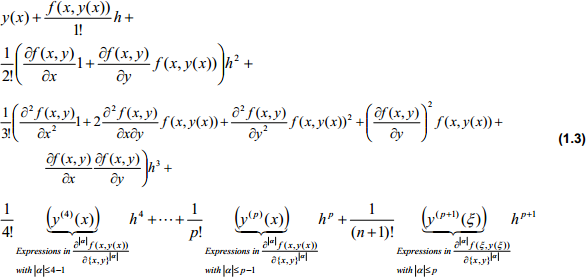
\includegraphics[width=10cm,trim=0cm 0cm 1.25cm 0cm,clip]{./bilder/ode_taylor_approx.png}
    %\end{minipage}\\
    
    
    
    
    \begin{minipage}{8cm}
      \subsubsection{Explizite Euler-Methode}
        Spezialfall der expliziten Methoden: Taylor mit Ordnung $p=1$. Relativ ungenaue Approximation,
        da hier die Ableitung pro Schritt unverändert bleibt. 
        
        Globaler Fehler: $\max_{0 \leq i \leq k} |y_i - y(x_i)|$ mit Anzahl Schritten $k$\\
        Lokaler Fehler: $y(x_n+h) - y_{n+1}$ wenn Initialwert des aktuellen Schritts is genau richtig
    \end{minipage}
    \hspace{8mm}
    \begin{minipage}{11cm}
      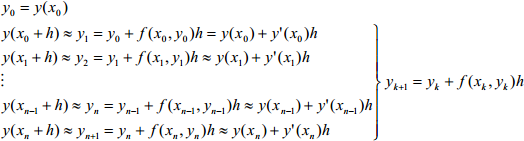
\includegraphics[width=10cm]{./bilder/ode_euler.png}
    \end{minipage}
      
    \subsubsection{Explizite Taylor-Methoden höherer Ordnung}
      Wenn $p > 1$ wird eine bessere Approximation erreicht. Allerdings steigt hier der rechnerische
      Aufwand enorm. Siehe Section \ref{sec:ode_explicit_methods} für Berechnung.
      
 \newpage     
    \skriptsubsubsection{Explizite Runge-Kutta (RK) Methoden}{8}
      Es werden $s$ rekursive Stages $k$ definiert, welche zusammenaddiert die Taylor-Approximation ergeben.
      Hier ist $s=4$
      \begin{align*}
        k_1 &= f(x,y)\\
        k_2 &= f(x + m h, y+m h k_1)\\
        k_3 &= f(x + n h, y+n h  k_2)\\
        k_4 &= f(x + p h, y+p h k_3) 
      \end{align*}     
      $$y(x+h) \approx y(x) + a h k_1 + b h k_2 + c h k_3 + d h k_4 $$ 
      Im Gegensatz zum Skript (S. 10) sind die 
      $h$ nicht in den $k$-Definitionen enthalten, sondern erst in der finalen Formel. Mit den richtigen Nebenbedingungen (S. 11) 
      entspricht diese Formel dem Taylor Polynom bis zur Ordnung 4
      
      Mit der Gleichsetzung zu Taylor definieren die expliziten RK-Methoden ein 
      überbestimmtes Gleichungssystem mit 8 Gleichungen und 7 Unbekannten $m,n,p$ und $a,b,c,d$.
      
      Es gibt daher verschiedene \textbf{Lösungen}, die hier auch für die Ordnung $s=2$ und $s=4$ aufgeführt sind:\\
      \begin{tabular}{lll}
        Name der Lösungen & \# Stages ($s$) & Lösungen\\
        Heun & 2 & $a=b=\frac12$, $m=1$ ($n=p=c=d=0$)\\
        Explicit Midpoint & 2 & $a=0$, $b=1$, $m=\frac12$ ($n=p=c=d=0$)\\
        Klassische Runge-Kutta & 4 & $m=n=\frac12$, $p=1$, $a=d=\frac16$, $b=c=\frac13$
      \end{tabular}
    
    \skriptsubsubsection{Generelles Framework für Runge-Kutta Methoden (Butcher Tableaus)}{13}
      \begin{minipage}{6cm}
        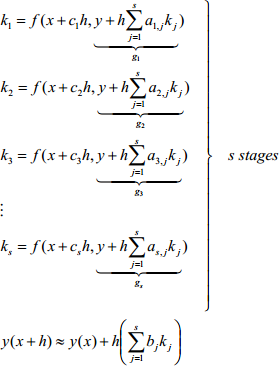
\includegraphics[width=5cm]{./bilder/ode_rungekutta_framework1.png}
      \end{minipage}
      \begin{minipage}{4.5cm}
        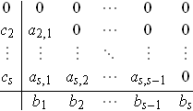
\includegraphics[width=3cm]{./bilder/ode_rungekutta_butcher.png}\\
        $\bm a$ = Aufteilung in $Y$\\
        $\bm b^T$ = Lösungen, durch Methode gegeben\\
        $\bm c$ = Aufteilung in $X$\\
        
        FSAL (First Same As Last) Spezialform:\\
        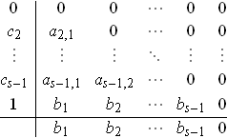
\includegraphics[width=3cm]{./bilder/butcher_fsal.png} 
      \end{minipage}
      \hspace{0.5cm}
      \begin{minipage}{9cm}
        Bedingungen (Für Explizite Methode): 
        \begin{liste}
          \item $c_i = \sum\limits_{j=1}^s a_{ij} = \sum\limits_{j=1}^{i-1} a_{ij}\,(i=2,\ldots,s)$
          \item $\sum\limits_{j=1}^s b_j = 1$
          \item $c_1=0$
          \item $a_{1j} = 0 \qquad 1\leq j\leq s $
          \item $a_{ij} = 0 \qquad j\geq i$
        \end{liste}
        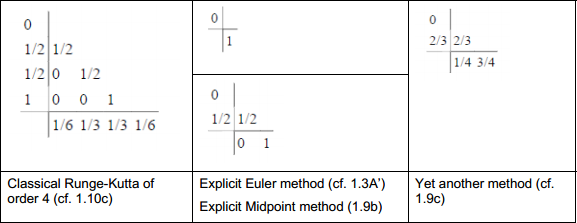
\includegraphics[width=8cm]{./bilder/ode_rungekutta_butcher_examples.png}\\
        Heun Methode (RK-2): $b_1 = b_2 = \frac{1}{2}; c_2=\frac{1}{2}; a_{2,1}=\frac{1}{2}$
      \end{minipage}
      
\newpage        
    \skriptsubsubsection{Adaptive Explizite Methoden}{17}
      Idee: Automatische Adaptierung der Step-Size $h$. Dies macht eine Definition des maximalen 
      Fehlers der Approximation nötig. Das \em Accuracy Goal \em ($ag$) 
      gibt die minimal übereinstimmende Anzahl Nachkommastellen an während
      das \em Precision Goal \em ($pg$) die Anzahl signifikanter Stellen des Resultats repräsentiert. 
      Der Toleranz-Paramter ist:
      $$\varepsilon = \varepsilon_a+ |y|\varepsilon_r=10^{-ag} + |y| 10^{-pg} \geq |e|.$$
     
      \subsubsubsection{Eingebettete Paare von expliziten Runge-Kutta Methoden}\\
        \begin{minipage}{5cm}
          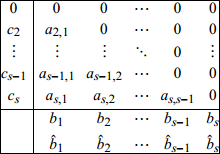
\includegraphics[width=4cm]{./bilder/ode_adaptive_butcher.png}
        \end{minipage}
        \begin{minipage}{13cm}
          Die Methode führt eine zweite Approximation, eine \em eingebettete Ordnung \em $\hat{p}$ 
          ein, welche für die Fehlerrechnung zuständig ist. Die \em primäre Ordnung \em $p$ wird 
          benötigt, um die Schrittweite zu berechnen. Meist ist $\hat{p} = p-1$.
          
          Das Butcher-Tableau wird dabei um eine Zeile der $b$-Zahlen erweitert.
        \end{minipage}\\
        
        Lokaler Fehler:
        $$e_n = y(x+h) - \hat{y}(x+h) = h_n \sum\limits_{j=1}^s (b_j - \hat{b}_j)k_j \Rightarrow 
        \Arrowvert e_n \Arrowvert = \left\Arrowvert h_n \sum\limits_{j=1}^s (b_j - \hat{b}_j)k_j \right\Arrowvert$$
          
        
        \begin{minipage}{7.5cm}
          Wenn bei aktuellem Schritt $\boxed{\frac{\Arrowvert e_n \Arrowvert}{\varepsilon} > 1}$, dann war die
          Schätzung von $h_n$ zu optimistisch und der Schritt muss mit kleinerer Schrittweite wiederholt
          werden (\textbf{Reject}). 
          
          Ansonsten $\boxed{\frac{\Arrowvert e_n \Arrowvert}{\varepsilon} \leq 1}$ wird fortgesetzt mit dem Update der Step-Size (\textbf{Proceed}): 
          
          $$h_{n+1} = h_n \left( \frac{\varepsilon}{\Arrowvert e_n \Arrowvert} \right)^{\frac{1}{\tilde{p}}}= 
          h_n \left( \frac{\Arrowvert e_n \Arrowvert}{\varepsilon} \right)^{-\frac{1}{\tilde{p}}}$$
          $$\varepsilon=\varepsilon_a+\varepsilon_r|y_n|
           \text{\qquad mit\quad} \tilde{p} = \min(p, \hat{p})+1 \text{ (Ordnung des Primärverfahrens)}$$
        \end{minipage}
        \hspace{0.5cm}
        \begin{minipage}{10.5cm}
          \subsubsubsection{Beispiel}\\
          \begin{tabular}{cccccc}
            \hline
            $x$ & $\bm y$ & $h_n$ & $\left( \frac{\Arrowvert e_n \Arrowvert}{\varepsilon} \right)^{-\frac{1}{\tilde{p}}}$ & $h_{n+1}$ & Status \\
            \hline
            $10$ & $[1, -1]^T$ & 1 & 0.4 & 0.4 & Reject\\
            10 & $[1,-1]^T$ & 0.4 & 1.5 & 0.6 & Proceed\\
            10.4 & $[0.420958, -1.40852]^T$ & 0.6 & 0.5 & 0.3 & Reject\\
            \hline
          \end{tabular}
        \end{minipage}
        
        
        
    \skriptsubsubsection{Stabilität von expliziten Methoden}{27}
      Globaler relativer Fehler darf nicht divergieren, d.h. muss beschränkt sein. 
      Da die Analyse mit zu untersuchender ODE wegen fehlender Kenntnis über die Lösung sehr schwierig
      ist, wird mit allgemeiner ODE gerechnet, dem Dahlquist Modell: 
      $$y' = A y \quad y(0) = 1 \qquad \text{mit } A = \Re\{A\} + j \Im\{A\} \in \mathbb{C}$$
      Dessen Lösung ist $y = e^{\Re\{A\} x} \left( \cos(\Im\{A\}x + j \sin(\Im\{A\} x) \right)$, also 
      eine Schwingung mit exponentieller Amplitude $e^{\Re\{A\} x}$ und Frequenz $\Im\{A\}$.
      
      Mit der zu untersuchenden Methode kann eine \em lineare Stabilitätsfunktion \em $F(z)$
      berechnet werden.
      
      \subsubsubsection{Beispiel} Anhand der Heun-Methode (RK-2) wird die Untersuchung gezeigt:
      \begin{align*}
        k_1 &= A y_k                                          & y_0 &= y(x_0) = y(0) = 1\\
        k_2 &= A(y_k + 1 h k_1) = A(y_k + Ah y_k) \qquad \Longrightarrow &
        y_{k+1} &= y_k \underbrace{\left(1 + hA + (hA)^2 \frac12\right)}_{F(hA) = F(z), \quad z=hA \in \mathbb{C}}
      \end{align*}
      Die lineare Stabilitätsfunktion kann jetzt auch so eingesetzt werden:
      $$y_{k+1} = \Big( | F(z) | \exp \big(j \arg(F(z))\big) \Big) y_k$$
      
      \begin{minipage}{10cm}
        Jetzt können drei Fälle unterschieden werden:
        \begin{liste}
          \item $\Re\{A\} < 0$: Die Amplitude der ODE wird exponentiell kleiner. Die Stabilitätsbedingung 
            verlangt, dass die approximierten Werte $y_k$ ($k=0,1,\ldots$) ebenfalls exponentiell 
            gedämpft werden. Daher und aus $y_{k+1} \propto | F(z) |$ folgt, dass $|F(z)| < 1$.
          \item $\Re\{A\} = 0$: Die Amplitude der ODE ist konstant 1. Die Stabilitätsbedingung 
            verlangt, dass die approximierten Werte $y_k$ ($k=0,1,\ldots$) ebenfalls konstant sind. 
            Daher und aus $y_{k+1} \propto | F(z) |$ folgt, dass $|F(z)| = 1$.
          \item $\Re\{A\} > 0$: Die Amplitude der ODE wird exponentiell grösser. Die Stabilitätsbedingung 
            verlangt, dass die approximierten Werte $y_k$ ($k=0,1,\ldots$) ebenfalls exponentiell 
            wachsen. Daher und aus $y_{k+1} \propto | F(z) |$ folgt, dass $|F(z)| > 1$.
        \end{liste}
        
        Die Fälle 2 und 3 bereiten keine Probleme (Bedingungen sind immer erfüllt), nur die erste Fall ist kritisch.
      \end{minipage}
      \hspace{1cm}
      \begin{minipage}{8cm}
        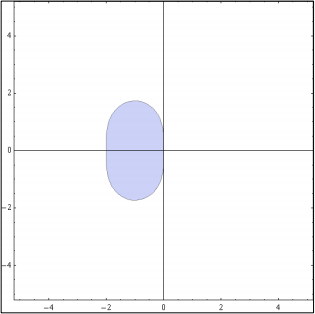
\includegraphics[width=6cm]{./bilder/ode_stability_heun.png}\\
        Fall 1 der Stabilitätsbedingung ($\Re\{A\} < 0$): \\
        $1 > |F(z)| = |1 + hA + \frac12 (hA)^2| \Rightarrow -2 < h \Re\{A\} < 0$.\\
        Fälle 2 und 3 sind in Abb. nicht berücksichtigt.
      \end{minipage}
      
      \vspace{1em}
      \subsubsubsection{Rekursive Formel} \formelbuch{29}
        Für das Stabilitätspolynom $F(z) = 1 + b_1 k_1(z) + \ldots + b_sk_s(z)$ existieren 
        rekursive Formeln:\\
        $k_1(z) = z, \qquad k_{j+1}(z) = z(1 + a_{j+1,1} k_1(z) + a_{j+1,2} k_2(z) + \ldots + a_{j+1,j} k_j(z))$
      
      \vspace{1em}
      \subsubsubsection{Schwäche der expliziten Methoden}: Stabilität!
    
    \skriptsubsubsection{Stiffness (Steifigkeit)}{33}
      Definition Stiffness = sehr schwierig (gemäss Wikipedia). Ungefähre Idee: Die expliziten 
      Methoden werden zu inakzeptabel kleinen Step-Sizes gezwungen (Computational complexity). 
      Dies trotz eigentlichen "`smoothen"' Oberflächen der Funktionen, die intuitiv nicht sehr 
      schwierig berechenbar sein sollten. \\
      
      Wenn Stabilitätsverletzungen (Stiffness) detektiert werden, soll zu 
      impliziten Verfahren (Blackbox-Solver) gewechselt werden, um dann mit non-Stiffness-Detektierung 
      zurück zu expliziten Verfahren umzustellen.\\
      
      Stiffness ist abhängig von:
      \begin{liste}
        \item Konkrete ODE
        \item Konkrete Schrittweite $h$
        \item Konkretes Verfahren (bspw. RK-4)
      \end{liste}
      
      \subsubsubsection{Stiffness Detektierung} 
        Voraussetzung: $c_{s-1} = c_s = 1$. Durch Testen von $\left|h \frac{\partial f(x,y)}{\partial y} \right|$ 
        auf die absolute Grenze der Stabilitätsregion kann
        Stiffness detektiert werden. Stiffness ist nicht erfüllt, wenn $|h \tilde{\lambda}|$ 
        ausserhalb des Stabilitätsbereich liegt.
        
        Beispiel explizite Runge-Kutta: 
        $$k_{s-1} = f(x+c_{s-1} h, \underbrace{y + h \sum\limits_{j=1}^s a_{s-1,j}k_j}_{g_{s-1}}) \qquad       
        k_{s} = f(x+c_{s} h, \underbrace{y + h \sum\limits_{j=1}^s a_{s,j}k_j}_{g_{s}}) \qquad 
        \Rightarrow \qquad \tilde{\lambda} = \frac{\Arrowvert k_s - k_{s-1} \Arrowvert}{\Arrowvert g_s - g_{s-1} \Arrowvert}$$
        
        $\tilde{\lambda}$ ist eine Schätzung für $f_y = \frac{\partial}{\partial y}f(x,y)$ z.B. $y'=x^4-25y^4=f(x,y)$ 
         und übernimmt die Rolle von $\Re \{A\}$ bei der Stabilitätsanalyse. 
        
        
  \skriptsubsection{Systeme von ODEs und ODEs höherer Ordnungen}{37}
    Systeme von ODEs werden in Vektor-Notation aufgeschrieben und wie üblich berechnet. 
    That's all.
    
  
\clearpage
\section{Ableitungstabelle}

\begin{center}
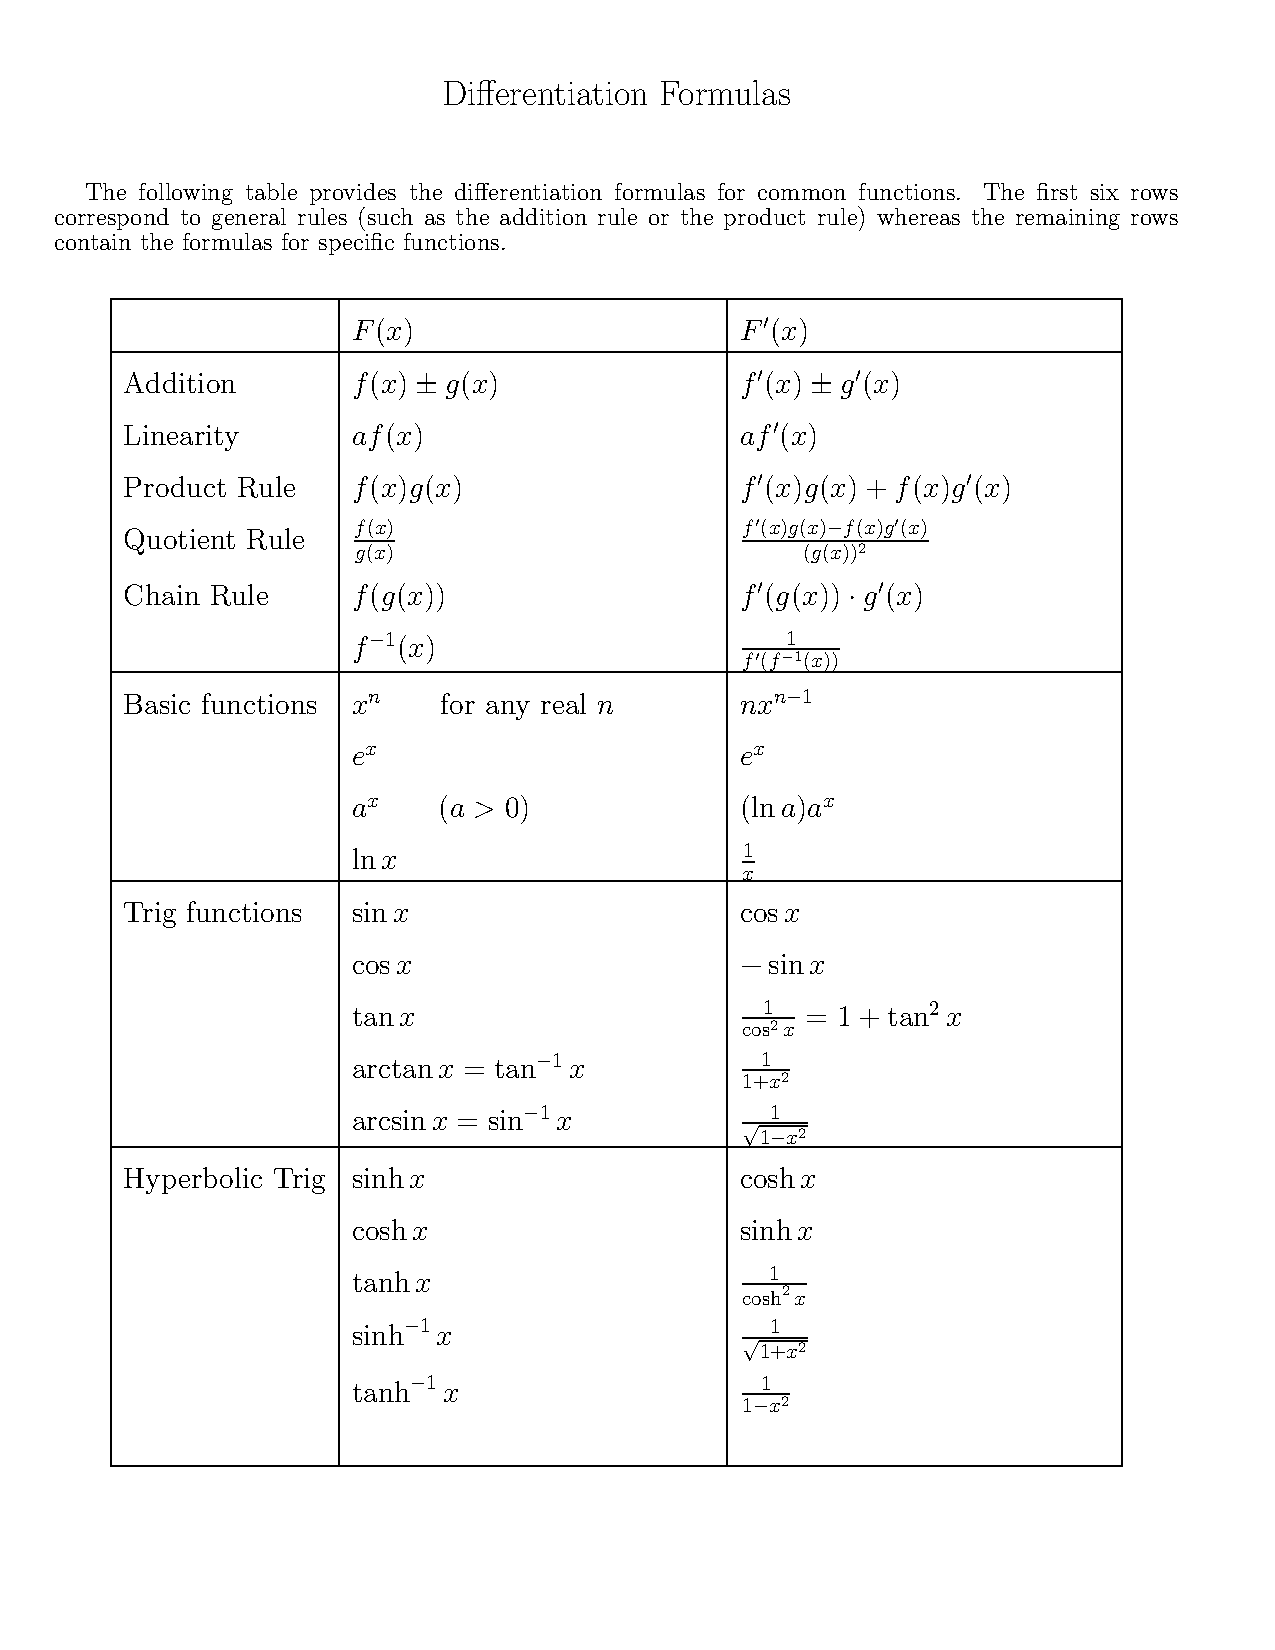
\includegraphics[page=1,width=14cm,trim=1.75cm 3.0cm 2.5cm 5.0cm,clip]{./files/calcrulz.pdf}
%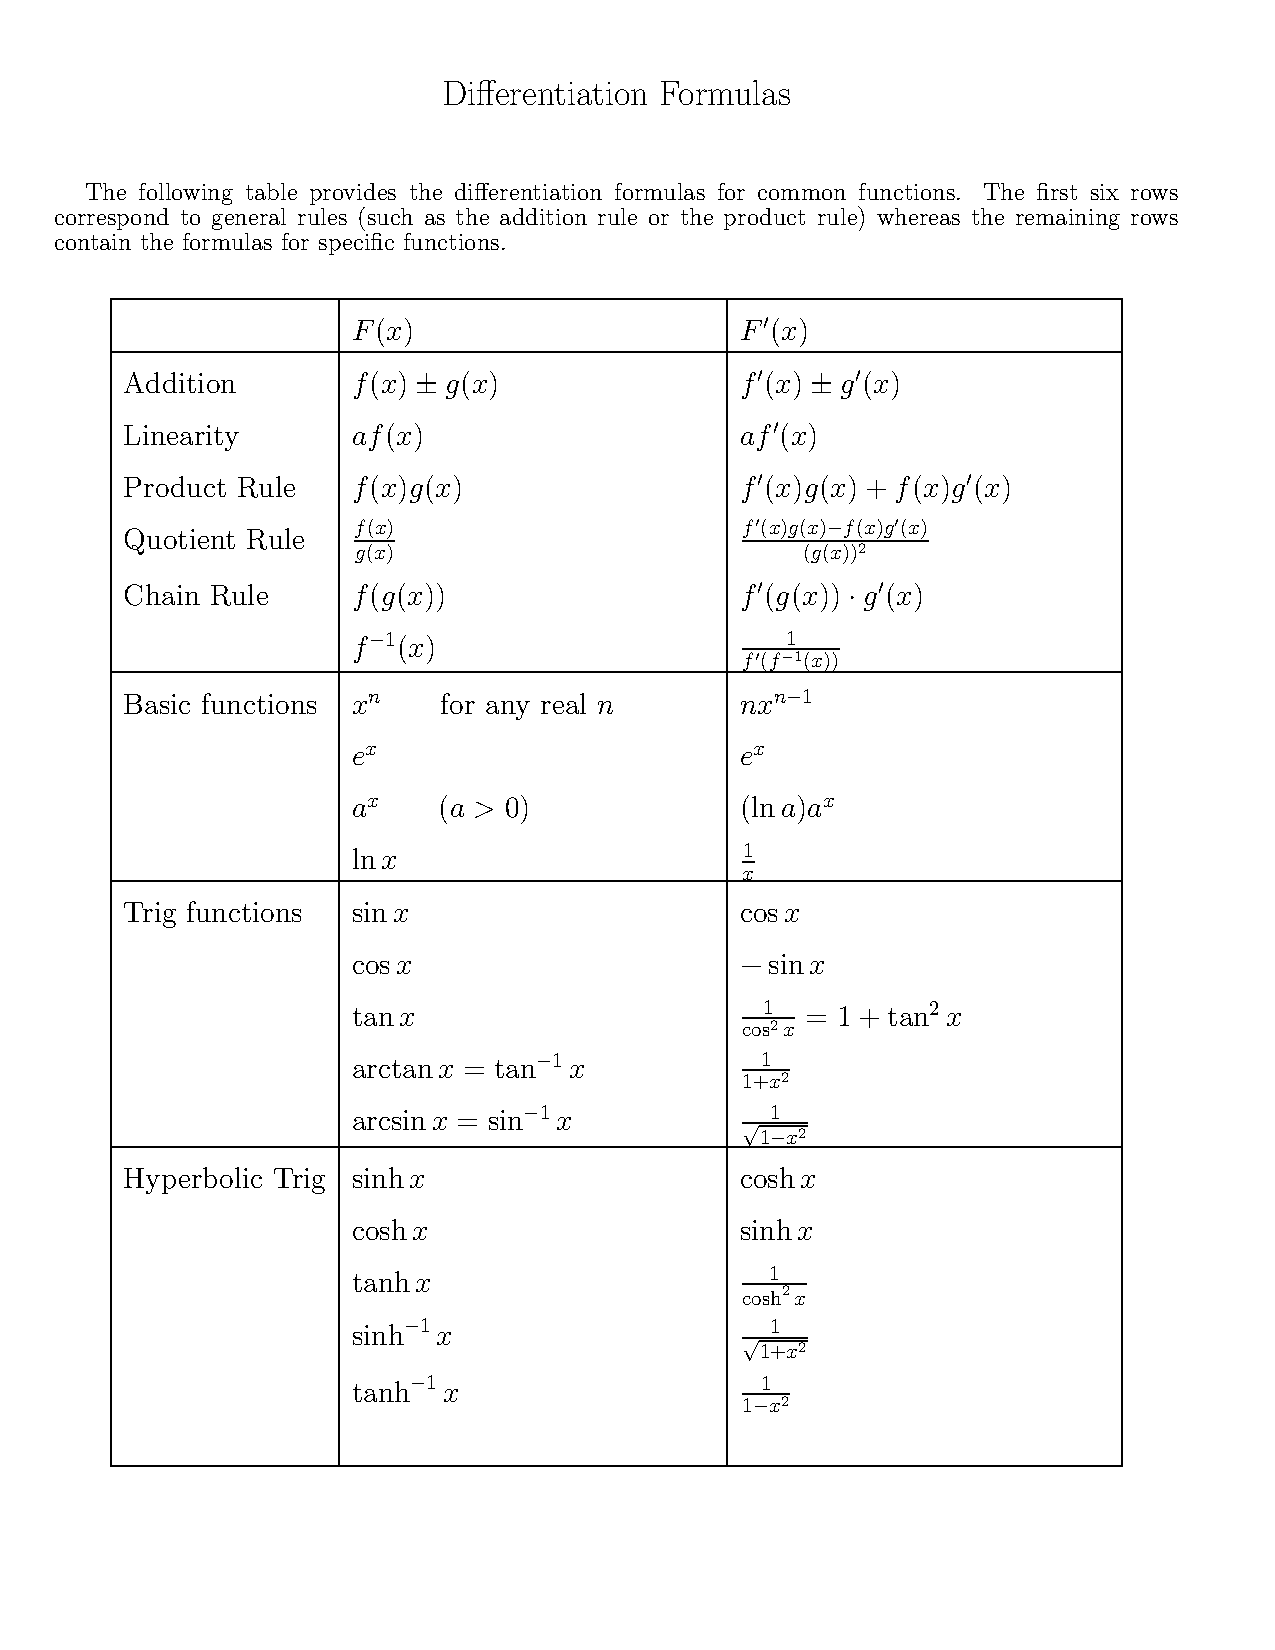
\includegraphics[page=1,width=14cm,clip]{./files/calcrulz.pdf}
\end{center}
\hfill
\section{Übersicht der Polynome}
\begin{tabular}{l|ll}
Name & Formel & Beispiel\\
\hline
Newton    & $\pi_n(x) =\prod_{i=1}^n(x-x_{i-1})$  & $\pi_2=(x-x_0)(x-x_1)$\\
Monomials & $x^n$                       & $x^2$\\
Bernstein & $B_{i,n}(x)=\binom{n}{i}(1-x)^{n-i} x^i$   & $B_{1,2}=2x(1-x)$\\
Chebyshev & $T_n(x)=\cos(n \arccos(x))$ & $T_2=2x^2-1$ 

\end{tabular}
\newpage

\section{Integrationstabelle}

\begin{center}
\includegraphics[page=2,width=18cm,trim=1.25cm 3cm 4.5cm 4cm,clip]{./files/calcrulz.pdf}
%\includegraphics[page=2,width=18cm,clip]{./files/calcrulz.pdf}
\end{center}


\end{document}
